\documentclass[11pt]{article}
\usepackage[margin=1.15in]{geometry}
\usepackage{amsmath,amssymb,amsthm}
\usepackage{booktabs}
\usepackage{longtable}
\usepackage{enumitem}
\usepackage{graphicx}
\usepackage{tikz}
\emergencystretch=3em
\usepackage[hidelinks]{hyperref}
\usepackage{xr-hyper}
\externaldocument[A1-]{paperA1}

\newtheorem{theorem}{Theorem}[section]
\newtheorem{lemma}[theorem]{Lemma}
\newtheorem{corollary}[theorem]{Corollary}
\newtheorem{proposition}[theorem]{Proposition}
\newtheorem{conjecture}[theorem]{Conjecture}
\theoremstyle{definition}
\newtheorem{definition}[theorem]{Definition}
\newtheorem{question}[theorem]{Question}
\theoremstyle{remark}
\newtheorem{remark}[theorem]{Remark}

\newcommand{\nd}[1]{\lVert #1\rVert}
\newcommand{\ML}{\mathrm{ML}}
\newcommand{\NN}{\mathbb{N}}
\newcommand{\ZZ}{\mathbb{Z}}
\newcommand{\RR}{\mathbb{R}}
\newcommand{\todo}[1]{\textbf{[AUTHOR TO CONFIRM: #1]}}
% number of an item of the companion paper [A1]
\newcommand{\xA}[1]{\ref{A1-#1}}

\title{An effective all-residue form of Kravitz's lemma, with applications to deleting one speed}
\author{Vico Bonfioli\thanks{This paper was produced with substantial assistance from AI systems (Anthropic's Claude models), working under the direction of the author, who reviewed the results and takes responsibility for the contents. Statements marked Lean-verified are checked by the Lean kernel, not by the author; see the section ``Use of AI'' before the references.}}
\date{Draft of 25 November 2026}

\begin{document}
\maketitle

\begin{abstract}
\noindent For a finite set $B$ of positive integers (speeds) let $\ML(B)=\max_{t}\min_{b\in B}\nd{tb}$, where $\nd{x}$ is the distance from $x$ to the nearest integer; the Lonely Runner Conjecture says $\ML\ge1/(N+1)$ for every set of $N$ speeds.
Kravitz showed that adding one very large speed $w$ to $B$ changes $\ML(B)$ by an explicit formula, but, except for a remark after his Lemma~9.4, he gave no size for ``very large'' and treated the added speed only in special residue classes.
We give two effective forms. Theorem~\ref{thm:K} is his Lemma~9.4 (the added speed is an integer at the top peaks, for instance a multiple of the lcm of their denominators): $\ML(B\cup\{w\})=wL/(w+v_\mu)$ for $w\ge2(\max B)^3$, with an upper bound for every admissible $w$. Theorem~\ref{thm:INS} is the all-residue form: a closed form $H_p(w)$ at each local maximum $p$ of the profile of $B$, the upper bound $\max_pH_p(w)$ for every positive integer $w$, and equality for $w\ge2M(M-1)$, where $M$ bounds the speeds of $B$. We evaluate both for $\{1,\dots,N\}$ with one speed $r\le N/2$ deleted, whose loneliness is Liu's value $2/D_0$ ($D_0$ the least integer $\ge N+1+r$ coprime to $r$): this gives the exact loneliness after a multiple $w\ge2N^2$ of $D_0$ is added (Theorem~\ref{thm:DEL}) and bounds for every $w\ge4N$ (Proposition~\ref{prop:G2}).

\medskip\noindent\textbf{Also.} The explicit thresholds and the bound for every $w$ are checked in Lean~4 (standard axioms; Theorem~\ref{thm:INS} in the form with a constant $c$); by hand are the identification of $c$ with the maximum over all peaks, the arc profile and the orientation of the two slopes in the deletion application. Table~\ref{tab:status} gives the status of every statement. This paper is readable alone; its companion~\cite{A1} cites it for two hand proofs and is used here only in Remark~\ref{rem:KV}.
\end{abstract}

\section{Introduction}\label{sec:intro}

\subsection{The picture in words}\label{sec:words}
\emph{What the paper is for.} It gives the effective, all-residue form of Kravitz's lemma on adding one very large speed to a set of speeds (Theorems~\ref{thm:K} and~\ref{thm:INS}) and applies it to deleting one speed from $[N]$ and adding one large speed (Theorem~\ref{thm:DEL}). The value $\ML([N]\setminus\{r\})=2/D_0$ of the deleted set is Liu's theorem and is not claimed here; what is added is the structure of the times at which it is attained and the exact value after one large speed is added. The motivation is the Lonely Runner Conjecture, $\ML\ge1/(N+1)$ for $N$ speeds, with equality for $[N]$: the $N$-sets that differ from $[N]$ in one entry are its nearest competitors, and their exact values show how close to $1/(N+1)$ the loneliness can come without being equal to it.

\emph{The picture.} For a set $B$ of speeds put $f_B(t)=\min_{b\in B}\nd{tb}$, the loneliness of the time $t$, so that $\ML(B)=\max_tf_B(t)$. A \emph{peak} of $B$ is a time $p$ at which $f_B$ has a local maximum, of height $\mu_p=f_B(p)$. Near a peak $f_B$ is a \emph{tent}: it rises with slope $\rho_p$ up to $p$ and falls with slope $\lambda_p$ after it, where $\rho_p$ and $\lambda_p$ are the speeds of the fastest runners that sit at distance $\mu_p$ from an integer at time $p$, one on each side. The \emph{equality times} are the peaks of greatest height $L=\ML(B)$. Now add a speed $w$. The new runner contributes the \emph{sawtooth} $t\mapsto\nd{wt}$, which at time $p+h$ equals $\nd{\theta+wh}$, where $\theta=wp\bmod1\in(-\frac12,\frac12]$ is its \emph{phase} at the peak. The loneliness of $B\cup\{w\}$ is the largest height at which the tent and the sawtooth are both present (Figure~\ref{fig:tent}). Near a peak this is the highest point where a side of the sawtooth, which has slope $\pm w$, meets a side of the tent; its height is a closed form $H_p(w)$ in $\mu_p,\rho_p,\lambda_p,\theta$ and $w$ (Section~\ref{sec:res}). When $w$ is large the sawtooth is steep, the point lies very close to $p$, no other runner of $B$ interferes, and $\ML(B\cup\{w\})$ is the largest $H_p(w)$ over the peaks.

\begin{figure}[ht]
\centering
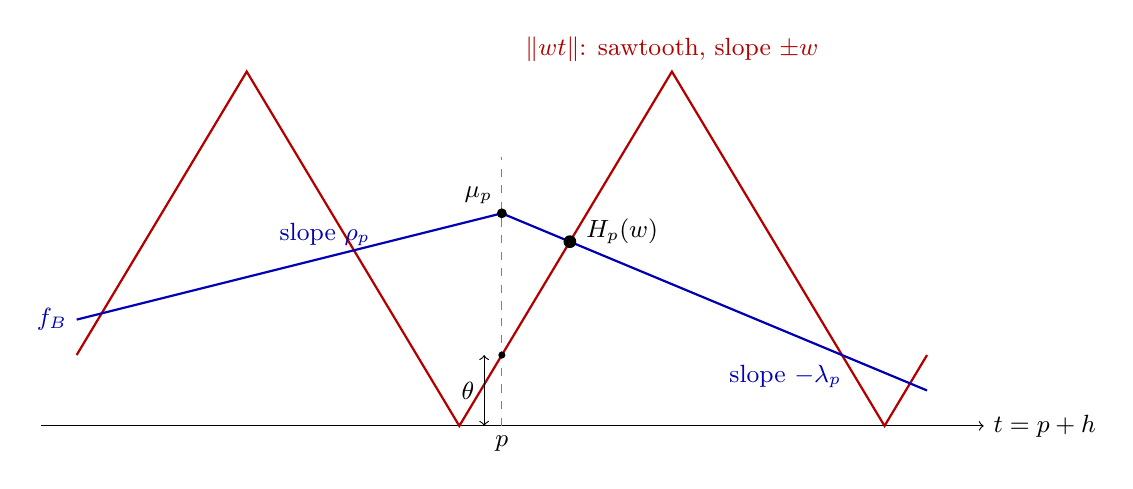
\begin{tikzpicture}[x=0.9cm,y=0.9cm,font=\small]
\draw[->] (-6.5,0) -- (6.8,0) node[right] {$t=p+h$};
\draw[dashed,gray] (0,0) -- (0,3.8);
\node[below] at (0,0) {$p$};
\draw[thick,red!70!black] (-6,1) -- (-3.6,5) -- (-0.6,0) -- (2.4,5) -- (5.4,0) -- (6,1);
\node[red!70!black,above] at (2.4,5) {$\nd{wt}$: sawtooth, slope $\pm w$};
\draw[thick,blue!70!black] (-6,1.5) -- (0,3) -- (6,0.5);
\node[blue!70!black,left] at (-6,1.5) {$f_B$};
\fill (0,3) circle (0.07) node[above left] {$\mu_p$};
\node[blue!70!black,above] at (-2.5,2.4) {slope $\rho_p$};
\node[blue!70!black,below] at (4.0,1.0) {slope $-\lambda_p$};
\fill (0.96,2.6) circle (0.09);
\node[right] at (1.05,2.75) {$H_p(w)$};
\draw[<->] (-0.25,0) -- (-0.25,1);
\node[left] at (-0.25,0.5) {$\theta$};
\fill (0,1) circle (0.05);
\end{tikzpicture}
\caption{A peak $p$ of $B$ (the tent $f_B$, in blue) and the sawtooth $\nd{wt}$ of an added speed $w$ (in red), schematic and not to scale. The sawtooth has height $\theta$ at $p$ (its phase) and slope $w$; the highest point under both curves has height $H_p(w)$, and $\ML(B\cup\{w\})$ is the largest such height over the peaks, for $w$ large.}
\label{fig:tent}
\end{figure}

\emph{The terms of the statements.} When the phase is $\theta=0$ at the equality times (that is, $wp$ is an integer there) one has Kravitz's case: $H_p(w)=w\mu_p/(w+\min(\rho_p,\lambda_p))$, and the loneliness is $wL/(w+v_\mu)$, where $v_\mu$ is the smallest of $\min(\rho_p,\lambda_p)$ over the equality times (Theorem~\ref{thm:K}). \emph{All-residue} means that Theorem~\ref{thm:INS} allows every phase $\theta$, that is, every residue of $w$ modulo the denominators of the peaks, with an explicit size for $w$; Kravitz's Lemma~10.1 treats arbitrary residues for $w$ sufficiently large and without a size. The \emph{descent lemma} (Kravitz's Lemma~8.4, Proposition~\ref{prop:descent}) says that if $B$ has $N-1$ speeds, $\ML(B)>1/N$ and $w\ge(2M-1)M$ with $M\ge\max B$, then $\ML(B\cup\{w\})\ge1/N$. The \emph{arc profile} (Lemma~\ref{lem:arc}) describes $f_B$ for $B=[N]\setminus\{r\}$ on an interval of times near a rational with denominator $r$: there $f_B$ is the minimum of two lines, a tent with peak $2/(2r+X)$ for a speed $X$ determined by the interval, which is how the value $2/D_0$ and the two slopes $2r$ and $D_0-2r$ are found. The \emph{one-entry value} is $\ML$ of $[N]$ with the speed $r$ replaced by $w$, that is, of $([N]\setminus\{r\})\cup\{w\}$.

\subsection{Background and summary}
The Lonely Runner Conjecture of Wills and Cusick~\cite{W} states that for any $N$ distinct positive integer speeds there is a time at which every runner on the unit circle is at distance at least $1/(N+1)$ from the starting point; in our notation $\ML(V)\ge1/(N+1)$ for every set $V$ of $N$ distinct positive integers, with equality for $V=[N]=\{1,\dots,N\}$. Kravitz~\cite{K} studied the values of $\ML$ just above this minimum by letting one speed become very large. If $B$ is a base and $w$ the added speed, then near a time $p$ at which $f_B$ has a local maximum the profile $f_B$ is a tent with two slopes, the added runner contributes a sawtooth of slope $w$, and $\ML(B\cup\{w\})$ is governed by the highest point under both. His Lemma~9.4 evaluates this for $w$ a sufficiently large multiple of the least common multiple of the denominators of the equality times, and his Lemma~10.1 for $w$ in an arbitrary residue class modulo that multiple, in both cases for $w$ sufficiently large and, except for a remark after Lemma~9.4, with no explicit size.

This paper makes these statements explicit with a size condition and extends the upper bound to every $w$. There are four results. (1) Theorem~\ref{thm:K}: Lemma~9.4 with the size $w\ge2(\max B)^3$, for an arbitrary base, together with an upper bound for every admissible $w$; Kravitz's Theorem~5.1 follows (Corollary~\ref{cor:K51}). (2) Theorem~\ref{thm:INS}: a closed form $H_p(w)$ at every local maximum $p$, an upper bound $\max_pH_p(w)$ for every positive integer $w$, and equality for $w\ge2M(M-1)$. (3) The Lipschitz bound and the descent lemma that accompany it are Kravitz's Proposition~8.1 and Lemma~8.4; Proposition~\ref{prop:descent} restates them in the forms checked in Lean. (4) For the base $[N]\setminus\{r\}$ with $r\le N/2$ the value $\ML=2/D_0$ is Liu's Theorem~18; Theorem~\ref{thm:DEL} adds the structure of the extremal times, the slopes $2r$ and $D_0-2r$, and the exact one-entry value, which is Theorem~\ref{thm:K} with its constants evaluated; Proposition~\ref{prop:G2} gives the second peak level, the threshold $2N^2$ and a bound for every $w\ge4N$. We believe that the pairing of the residue terms in the arXiv~v1 print of Kravitz's Lemma~10.1 is swapped relative to its own definitions; the published version may differ.\footnote{Reference: \cite[p.~19]{K}; we have not seen the published version, and Theorem~\ref{thm:INS} does not depend on how the printed lemma is read. Check in three lines, in exact rational arithmetic, for $B=\{1,4\}$, $\ML(B)=2/5$ and added speed $v_n=12$: (1) the printed pairing gives $(2v_n-1)/(5(v_n+1))=23/65$; (2) at $t=5/13$ the distances of the speeds $1,4,12$ are $5/13$, $6/13$, $5/13$; (3) hence $\ML(1,4,12)\ge5/13=25/65>23/65$. The general computation is in Appendix~\ref{sec:appsign}.}

This paper is readable alone. A companion paper~\cite{A1} applies the same picture to the sets obtained from $[N]$ by replacing one speed $r>N/2$ by a multiple $mr$, and to related questions on added speeds; it cites this paper for the hand proofs of its Proposition~\xA{prop:allw} and Theorem~\xA{thm:exact} (here Theorem~\ref{thm:DEL}(e) and Proposition~\ref{prop:G2}), and this paper uses it only in Remark~\ref{rem:KV}, which derives the main formula of that paper (its Theorem~\xA{thm:V}) from Theorem~\ref{thm:K}.

\subsection{Conventions and notation}
For a finite set $V\subset\ZZ_{>0}$ put
\[
f_V(t)=\min_{v\in V}\nd{tv},\qquad \ML(V)=\max_{t\in\RR}f_V(t),
\]
where $\nd{x}$ is the distance from $x$ to the nearest integer; the maximum exists because $f_V$ is continuous and $1$-periodic, so $t$ may be taken in $\RR/\ZZ$. Since $t\mapsto ct$ is a bijection of $\RR$, $\ML(cV)=\ML(V)$ for integers $c\ge1$; and $V\subseteq V'$ implies $\ML(V)\ge\ML(V')$. An $N$-set is a set of $N$ distinct positive integers, and $[N]=\{1,\dots,N\}$. Here $N$ is the number of speeds of the set after the change: in Theorem~\ref{thm:DEL} the base $[N]\setminus\{r\}$ has $N-1$ speeds and the set with $w$ added or substituted has $N$; in Proposition~\ref{prop:descent}, $|B|=N-1$. The letter $n$ means $N+1$ in Goddyn--Wong~\cite{GW} and Zhang~\cite{Z}, and $N$ in Fan--Sun~\cite{FS} and Kravitz~\cite{K}; this paper uses $N$ only. In the Lean development (Section~\ref{sec:lean}) $k$ indexes vectors of length $k+1$; the letter $k$ is used in the body of the paper only as part of Lean names. The \emph{loneliness} of a time $t$ is $f_V(t)$ and $\ML(V)$ is the maximum loneliness; a \emph{peak} of $B$ is a local maximum of $f_B$ (Section~\ref{sec:res}).

\begin{samepage}
\paragraph{Notation.}\nopagebreak
\begin{center}
\small
\begin{tabular}{l p{0.68\textwidth}}
\toprule
symbol & meaning \\
\midrule
$\nd{x}$, $\ML(V)$ & distance to the nearest integer; $\max_t\min_{v\in V}\nd{tv}$ \\
$[N]$ & $\{1,\dots,N\}$ \\
$B$, $M$, $f$, $L$ & base set, $\max B$ (or any upper bound of $B$), $f(t)=\min_{b\in B}\nd{tb}$, $L=\max f$ (Theorem~\ref{thm:K}) \\
$E$, $\rho_p$, $\lambda_p$ & equality times $\{p:f(p)=L\}$; largest speeds at $+L$, at $-L$ at time $p$ \\
$v_\mu$, $L_2$, $K(w)$ & $\min_{p\in E}\min(\rho_p,\lambda_p)$, one number for each base $B$ (the subscript is Kravitz's notation); second peak level: the largest value below $L$ of $f$ at a local maximum; $wL/(w+v_\mu)$ \\
$p$, $\mu_p$, $\rho_p,\lambda_p$ & peak (local maximum of $f$), its height; fastest speeds at $+\mu_p$, $-\mu_p$ (Section~\ref{sec:res}) \\
$\theta_p(w)$, $H_p(w)$ & phase $wp\bmod1$; tent-against-sawtooth height (Section~\ref{sec:res}) \\
$r$, $D_0$, $D_1$ & removed speed, $1\le r\le N/2$; least integers $\ge N+1+r$, resp.\ $>D_0$, coprime to $r$ (Section~\ref{sec:del}) \\
$a$, $X_0$ & $ra\equiv1\pmod{D_0}$ (the equality times of $[N]\setminus\{r\}$ are $\pm a/D_0$); $X_0=D_0-2r$ (Theorem~\ref{thm:DEL}); for $B=[N]\setminus\{r\}$ the number $v_\mu$ equals $\min(2r,X_0)$ (Theorem~\ref{thm:DEL}(d)) \\
\bottomrule
\end{tabular}
\end{center}
\end{samepage}

\subsection{Results}\label{sec:res}
Three statements are made in this section: Theorem~\ref{thm:K} for a base $B$ and an added speed that is an integer at every equality time, Theorem~\ref{thm:INS} for an arbitrary added speed, and Theorem~\ref{thm:DEL} for the base $[N]\setminus\{r\}$. Proofs are in Sections~\ref{sec:K}, \ref{sec:INS} and~\ref{sec:del}.

\begin{theorem}[Kravitz's lemma, effective two-level form]\label{thm:K}
Let $B$ be a finite set of positive integers, $M=\max B$, $f(t)=\min_{b\in B}\nd{tb}$ and $L=\max f$ with $0<L<\tfrac12$. Let $E=\{t\in\RR/\ZZ: f(t)=L\}$ (the equality times; a finite set of rationals). For $p\in E$ let $\rho_p=\max\{b\in B: bp\equiv L\pmod 1\}$ and $\lambda_p=\max\{b\in B:bp\equiv-L\pmod 1\}$, and let $v_\mu=\min_{p\in E}\min(\rho_p,\lambda_p)$. Let $L_2$ be the largest value $<L$ taken by $f$ at a local maximum ($L_2=0$ if there is none). For an integer $w\ge1$ put $K(w)=wL/(w+v_\mu)$. If $wp\in\ZZ$ for every $p\in E$ then:
\begin{enumerate}[label=(\alph*),nosep]
\item $\ML(B\cup\{w\})\le\max(K(w),L_2)$, with no condition on the size of $w$;
\item if $w\ge2M^3$ (that is, $w\ge2(\max B)^3$) then $\ML(B\cup\{w\})=K(w)=wL/(w+v_\mu)$.
\end{enumerate}
\end{theorem}
The hypothesis ``$wp\in\ZZ$ for every $p\in E$'' holds, for instance, when $w$ is a multiple of the least common multiple $D$ of the reduced denominators of the elements of $E$, and in fact only then (Corollary~\ref{cor:K94}). Theorem~\ref{thm:K} contains the case $B=[N-1]$ (Corollary~\ref{cor:K51}, Kravitz's Theorem~5.1) and, through Remark~\ref{rem:KV}, Theorem~\xA{thm:V} of the companion paper~\cite{A1}; Theorem~\ref{thm:INS} extends its upper bound to every $w$ and its equality statement to every residue of $w$.

\paragraph{Definitions.}
Let $B$ be a finite set of positive integers and $f(t)=\min_{b\in B}\nd{tb}$. A \emph{peak} of $B$ is a real $p$ at which $f$ has a local maximum, with $\mu_p:=f(p)\in(0,\frac12]$; integer translates of peaks are peaks, and the equality times of Theorem~\ref{thm:K} are the peaks with $\mu_p=\ML(B)$. Put $\rho_p=\max\{b\in B: bp\equiv\mu_p\pmod1\}$ and $\lambda_p=\max\{b\in B:bp\equiv-\mu_p\pmod1\}$; both sets are nonempty (Lemma~\ref{lem:loc}(a); for $\mu_p=\frac12$ every $b\in B$ has $bp\equiv\frac12$ and $\rho_p=\lambda_p=\max B$). Note that $\rho_p$ is the speed of the fastest runner at $+\mu_p$, which is the \emph{left} slope of the tent, and $\lambda_p$ the right slope, as in Lemma~\ref{lem:loc}(b). For a positive integer $w$ let $\theta=\theta_p(w)\in(-\frac12,\frac12]$ with $wp\equiv\theta\pmod1$, and
\[
H_p(w)=\begin{cases}\mu_p&\text{if }|\theta|\ge\mu_p,\\[2pt]\max\Bigl(\dfrac{w\mu_p+\lambda_p\theta}{w+\lambda_p},\ \dfrac{w\mu_p-\rho_p\theta}{w+\rho_p}\Bigr)&\text{if }|\theta|<\mu_p.\end{cases}
\]
Then $H_p(w)\le\mu_p$, with strict inequality when $|\theta|<\mu_p$ (each of the two terms is a weighted mean of $\mu_p$ and a number below $\mu_p$, or is at most $|\theta|$), and for $\theta=0$ one has $H_p(w)=w\mu_p/(w+\min(\rho_p,\lambda_p))$. The peak set is finite modulo $1$: peaks with $\mu_p<\frac12$ have denominators $\le2M-1$ (Lemma~\ref{lem:loc}(c)), and a peak with $\mu_p=\frac12$ satisfies $(\max B)p\equiv\frac12$. Lemma~\ref{lem:loc} was stated under the standing assumption $\ML(B)<\frac12$; it is used here for peaks with $\mu_p<\frac12$, and a peak with $\mu_p=\frac12$ is treated directly, since every runner is then at $\frac12$ and $f(p+h)=\frac12-(\max B)|h|$ near $p$.

\begin{theorem}[Insertion of one speed]\label{thm:INS}
Let $B$ be a finite set of positive integers, $M\ge\max B$ an integer, and $w$ a positive integer (it may already lie in $B$).
\begin{enumerate}[label=(\alph*),nosep]
\item (lower bound) $\ML(B\cup\{w\})\ge\dfrac{w\,\ML(B)}{w+M}$.
\item (upper bound) Let $c>0$ be a real number such that $H_p(w)\le c$ for every peak $p$ with $\mu_p>c$. Then $\ML(B\cup\{w\})\le c$. In particular $\ML(B\cup\{w\})\le\max_pH_p(w)$.
\item (equality) If $\ML(B)<\frac12$ and $w\ge2M(M-1)$, then $\ML(B\cup\{w\})=\max_pH_p(w)$. That is: if $c$ bounds $H_p(w)$ above $c$ as in (b) and $c=H_p(w)$ for some peak $p$, then $\ML(B\cup\{w\})=c$.
\end{enumerate}
No divisibility, primitivity or injectivity hypothesis is made on $B$ or $w$ in (a) and (b); in (c) the bound $M$ is any upper bound of the entries.
\end{theorem}
Part (b) is the extension of the upper bound of Theorem~\ref{thm:K}(a) to every $w$: if $wp\in\ZZ$ at the equality times, then $c=\max(K(w),L_2)$ satisfies the hypothesis of (b) (equality peaks have $H_p=w\mu_p/(w+\min(\rho_p,\lambda_p))\le K(w)$, and the other peaks have $H_p\le\mu_p\le L_2$), which recovers Theorem~\ref{thm:K}(a) (by hand). In Lean, (b) and the second form of (c) are \texttt{ML\_snoc\_le\_Hform} and \texttt{ins\_E} with a number $c$ as in the statement; the maximum over peaks (finiteness of the peak set) is by hand. Part (a) is \texttt{ML\_snoc\_ge\_LIP}. In all of them $w$ is an integer, because \texttt{Fin.snoc v w} appends an integer; the corresponding statements for real $w>0$ are by hand (the proofs use no integrality of $w$).

\paragraph{Relation between Theorems~\ref{thm:K} and~\ref{thm:INS}.}
Theorem~\ref{thm:INS} is the general statement: it holds for every positive integer $w$, whatever its phase $\theta_p(w)$ at the peaks. Theorem~\ref{thm:K} is the case in which the phase is $0$ at every equality time, that is $wp\in\ZZ$ for $p\in E$, which holds exactly when $w$ is a multiple of the lcm $D$ of the reduced denominators of $E$ (Corollary~\ref{cor:K94}). In that case $H_p(w)=wL/(w+\min(\rho_p,\lambda_p))$ at an equality time and the largest of these is $K(w)=wL/(w+v_\mu)$, so part (a) of Theorem~\ref{thm:K} follows from Theorem~\ref{thm:INS}(b) (by hand, as shown above). Part (b) of Theorem~\ref{thm:K}, the equality $\ML(B\cup\{w\})=K(w)$ for $w\ge2(\max B)^3$, has its own Lean statement, with the term $L_2$ for the peaks below the top. Theorem~\ref{thm:INS}(c) gives equality for $w\ge2M(M-1)$ in every residue class; in Lean it is stated in the characterised form with a number $c$, and the identification of $c$ with the maximum of $H_p(w)$ over all peaks is by hand.

\paragraph{The four sizes.}
``Very large'' means four different numbers in this paper, because the four statements compare different things. Each size is a condition on the added speed $w$ for which a stated conclusion holds; $M$ is an upper bound of $\max B$ and, for the base $[N]\setminus\{r\}$ of Theorem~\ref{thm:DEL}, $M=N$.
\begin{center}
\small
\begin{tabular}{l p{0.25\textwidth} p{0.29\textwidth} p{0.17\textwidth}}
\toprule
size of $w$ & applies to & conclusion & where \\
\midrule
$2M(M-1)$ & any base $B$ with $\ML(B)<\frac12$; every residue of $w$ & $\ML(B\cup\{w\})=\max_pH_p(w)$ (max over all peaks) & Thm~\ref{thm:INS}(c) \\
$2M^3=2(\max B)^3$ & any base $B$; $wp\in\ZZ$ at every equality time (e.g.\ $D\mid w$) & $\ML(B\cup\{w\})=K(w)=wL/(w+v_\mu)$ (the equality times win) & Thm~\ref{thm:K}(b) \\
$2N^2$ & $B=[N]\setminus\{r\}$, $r\le N/2$, $D_0\mid w$ & $\ML=2w/(D_0(w+v))$ & Thm~\ref{thm:DEL}(e), Prop.~\ref{prop:G2}(ii) \\
$4N$ & $B=[N]\setminus\{r\}$, every integer $w\ge4N$ & two-sided bounds $\frac{2w}{D_0w+4rX_0}\le\ML\le\frac2{D_0}$, not a value & Prop.~\ref{prop:G2}(iii) \\
\bottomrule
\end{tabular}
\end{center}
The first two apply to an arbitrary base and are the same comparison at two levels. The size $2M(M-1)$ is what the lower bound at a single peak needs, $w\ge(d_p-1)M$ with $d_p\le2M-1$ the denominator of $p$ (Lemma~\ref{lem:peakL}); it makes no comparison between different peaks, so the value is the maximum of $H_p(w)$ over all peaks. The size $2M^3$ adds that the equality times win over the other peaks: $K(w)\ge L_2$ holds iff $w(L-L_2)\ge L_2v_\mu$, and since $L-L_2\ge(2M-1)^{-2}$ (Lemma~\ref{lem:loc}(c)) and $L_2v_\mu<M/2$, it holds as soon as $w\ge\frac12M(2M-1)^2$, which is below $2M^3$ (Lemma~\ref{lem:thr}). For $2M(M-1)\le w<2M^3$ Theorem~\ref{thm:INS}(c) still gives the value as the maximum of $H_p(w)$ over all peaks, without the identification with $K(w)$; this is why Theorem~\ref{thm:K}(a) carries the term $L_2$. For the base $[N]\setminus\{r\}$ the second peak level $L_2$ is known ($2/D_1$ or $\frac1{N+1}$, Proposition~\ref{prop:G2}(i)), which replaces the bound $L-L_2\ge(2M-1)^{-2}$ and lowers $2M^3=2N^3$ to $2N^2$ (for $M=N$, $2N^2=2M(M-1)+2N$); the exact condition is $w\ge\max(2N-v_\mu,\lceil v_\mu D_0/\Delta\rceil)$, which is at most $2N^2$. The size $4N$ concerns every $w$, not only multiples of $D_0$: there the exact value is not given, only the two-sided bound, and the Lean statement needs $w\ge4N$ (the hand proof needs only $w\ge w_G$ with $w_G\le3N$).

\paragraph{Worked instance.}
$B=\{1,2,3,5\}$, $M=5$, $\ML(B)=\frac14$. The top peaks are $p=\frac14$ and $p=\frac34$ with $\mu=\frac14$. At $p=\frac14$ the speeds $1$ and $5$ are at $+\frac14$ (as $\frac54\equiv\frac14$), so $\rho=5$, and the speed $3$ is at $-\frac14$ (as $\frac34\equiv-\frac14$), so $\lambda=3$; at $p=\frac34$ the two are exchanged. The other peaks have $\mu\le\frac16$. For $w=40=2M(M-1)$ one has $wp=10\in\ZZ$ at $p=\frac14$, so $\theta=0$ and $H=\frac{40\cdot\frac14}{40+3}=\frac{10}{43}$; at $p=\frac34$ also $\theta=0$ and $H=\frac{10}{43}$ (the smaller of $\rho,\lambda$ is again $3$); the lower peaks have $H\le\mu\le\frac16<\frac{10}{43}$. So $\ML(1,2,3,5,40)=\frac{10}{43}$ (the value agrees with an exact computation). For $w=41$ one has $\theta=\frac14=\mu$, so $H=\frac14$ and $\ML(1,2,3,5,41)=\frac14$, although $41$ is not a multiple of the denominator $4$: Theorem~\ref{thm:K} does not apply, Theorem~\ref{thm:INS}(c) does.

\begin{theorem}[Deletion value, equality times and one-entry value]\label{thm:DEL}
Let $N\ge3$ and $1\le r\le N/2$, let $D_0$ be the least integer $\ge N+1+r$ coprime to $r$, let $B=[N]\setminus\{r\}$ with $f_B(t)=\min_{b\in B}\nd{tb}$, and put $X_0=D_0-2r$ and $v=\min(2r,X_0)$.
\begin{enumerate}[label=(\alph*),nosep]
\item Every vector of positive integers whose set of entries is $[N]\setminus\{r\}$ (repeats and order allowed) has $\ML=2/D_0$. For every vector whose entries lie in $[N]\setminus\{r\}$, $\ML\ge2/D_0$.
\item The real $p$ with $f_B(p)=2/D_0$ are exactly $p=\pm a/D_0+\ZZ$ with $ra\equiv1\pmod{D_0}$.
\item At each such $p$ all runners at $+2/D_0$ have one speed and all runners at $-2/D_0$ have the other, the two speeds being $2r$ and $D_0-2r$, and both sides are occupied.
\item $v$ is the number $v_\mu$ of Theorem~\ref{thm:K} for the base $B$ (this is the only meaning of $v_\mu$ in this paper): (V1) every equality time has a runner of speed $\ge v_\mu$ at $+2/D_0$ and one at $-2/D_0$, and (V2) at some equality time all runners on one side have speed $\le v_\mu$; these two properties determine $v_\mu$, and $v_\mu=v$.
\item If $D_0\mid w$ and $w\ge2N^2$, then $\ML\bigl(B\cup\{w\}\bigr)=\dfrac{2w}{D_0\,(w+v)}$, where $B\cup\{w\}$ is $[N]$ with the entry $r$ replaced by $w$. (Theorem~\ref{thm:K}(b) gives this for $w\ge2N^3$; Proposition~\ref{prop:G2}(ii) lowers the threshold to $2N^2$.)
\end{enumerate}
\end{theorem}
All five statements are verified in Lean (Table~\ref{tab:status}): (a) is \texttt{ML\_ge\_delB}, \texttt{ML\_eq\_two\_div}; (b) is \texttt{eqtime\_classify} and \texttt{gap\_eq\_at\_inv}; (c) is \texttt{runners\_at\_eq}; (d) is \texttt{V1\_holds}, \texttt{V2\_holds}, \texttt{vmu\_eq}; (e) is \texttt{one\_entry\_value\_2N2\_dFam} for $w\ge2N^2$ (and \texttt{one\_entry\_value}, \texttt{one\_entry\_value\_dFam} for $w\ge2N^3$). Three points on the form of the Lean statements. First, \texttt{runners\_at\_eq} states the \emph{unordered} pair $\{2r,D_0-2r\}$; that $2r$ is the speed at $+2/D_0$ when $p=a/D_0$ (and $D_0-2r$ at $-2/D_0$, the two exchanged at $-a/D_0$) is the ordered refinement, which is in the proof and is not a Lean statement. Second, in (e) the Lean vector is \texttt{wFam (k+1) r w} with $N=k+2$ entries, namely $(1,\dots,N)$ with the entry $r$ replaced by $w$; its set of entries is $B\cup\{w\}$, and $w\ge2N^3>N$ is never a repeat. This $N$ is the $N$ of the companion paper~\cite{A1} (its \texttt{OE\_low\_unconditional} has $k+1=N$ entries in its vector). Third, (a) is stated in Lean for \texttt{DSpec N r D}, whose conditions are exactly $1\le r$, $2r\le N$, $3\le N$, $D\ge N+1+r$, $\gcd(D,r)=1$ and minimality of $D$.

\paragraph{Worked instance.}
$N=14$, $r=3$: $N+1+r=18$ is divisible by $3$ and $19$ is not, so $D_0=19$ and $\ML([14]\setminus\{3\})=\frac2{19}$. The congruence $3a\equiv1\pmod{19}$ gives $a=13$, and the equality times modulo $1$ are $\frac{13}{19}$ and $\frac6{19}$. At $\frac{13}{19}$ the only retained speed with $13x\equiv2\pmod{19}$ is $x=6=2r$ (runner at $+\frac2{19}$) and the only one with $13x\equiv-2$ is $x=13=D_0-2r$ (runner at $-\frac2{19}$), so $v_\mu=6$. For $w=5491=19\cdot289$, which is $\ge2N^3=5488$ and a fortiori $\ge2N^2=392$, (e) gives $\ML=\frac{2\cdot5491}{19\cdot5497}=\frac{578}{5497}$; this agrees with an exact computation. (The threshold $2N^3$ is not sharp here: the multiples $570$, $1900$ and $5472$ of $19$, all $\ge2N^2$, also satisfy the formula.)


\subsection{Idea of the proofs}
Fix a base $B$ and write $f=f_B$. Near a peak $p$ the function $f$ lies under a tent with slope $\rho_p$ on the left and $-\lambda_p$ on the right, where $\rho_p$ and $\lambda_p$ are the speeds of the fastest runners at distances $+\mu_p$ and $-\mu_p$ from an integer at time $p$. An added speed $w$ contributes the sawtooth $\nd{\theta+wh}$ at time $p+h$, where $\theta=wp\bmod1$ is its phase at the peak, and $\ML(B\cup\{w\})$ is the height of the highest point under both. Theorem~\ref{thm:K} is this picture at the top peaks: near an equality time $f$ falls at slope at least $v_\mu$ on both sides, and a speed $w$ that is an integer at the peak cuts all peaks at one height, namely $wL/(w+v_\mu)$. For Theorem~\ref{thm:INS}: at every peak the old profile is a tent, the added speed is a sawtooth with a known phase, and the highest point under both is $H_p(w)$; for $w$ large the crossing is so close to the peak that no old runner can interfere. For Theorem~\ref{thm:DEL}: Dirichlet's theorem forces any time at which $f_B>\frac1{N+1}$ onto an arc where the profile is a tent made of two lines, the rising speed $2r$ and the falling largest retained speed $X$ of one residue class, with peak $2/(2r+X)$; the smallest admissible $2r+X$ is $D_0$, a rational witness time attains $2/D_0$, and the same two lines are the slopes at the top peak that Theorem~\ref{thm:K} needs.

\subsection{Status of every statement}
Table~\ref{tab:status} gives for each statement whether it is verified in Lean~4 (standard axioms), proved by hand, computed or conjectured. In Lean: Theorem~\ref{thm:K}; Corollary~\ref{cor:K51}; Theorem~\ref{thm:INS} for integer $w$, with (b) and (c) in the form with a number $c$ (the maximum over all peaks, which needs finiteness of the set of peaks, is by hand); Proposition~\ref{prop:descent}, whose last sentence is conditional on \texttt{LRCHyp}; \texttt{LRCHyp} is a hypothesis predicate (the Lonely Runner statement for the relevant number of speeds), never instantiated in the development, so that sentence is not an unconditional Lean statement; Theorem~\ref{thm:DEL} except the ordered orientation of the two slopes in (c); and in Proposition~\ref{prop:G2} the bound on $L_2$, the one-entry value with threshold $2N^2$ and the lower bound for $w\ge4N$. By hand only: the arc profile, $D_0\le2N-1$, the remaining parts of Proposition~\ref{prop:G2}, the real-$w$ forms, Remark~\ref{rem:KV} and Remark~\ref{rem:sign}. Computed, not proved: Conjecture~\ref{conj:M2} (threshold $(\max B)^2$). The statements are unrefereed; the state of the literature search is in Section~\ref{sec:prior}.
{\footnotesize
\setlength{\tabcolsep}{4pt}
\begin{longtable}{@{}p{0.19\textwidth}p{0.27\textwidth}p{0.47\textwidth}@{}}
\caption{Status per statement. ``Lean'': the declarations named build in the library, contain no \texttt{sorry}, and \texttt{\#print axioms} prints only the three standard axioms (saved build outputs, read; no clean-checkout rebuild has been done). ``Reviewed'': re-derived by hand by a second pass that did not write the proof; this is not a referee's reading. In Lean names \texttt{KStar} refers to the files of Theorem~\ref{thm:K}, and \texttt{Fin.snoc v w} appends the speed $w$ to $v$.}\label{tab:status}\\
\toprule
statement & status & Lean declarations (axioms: \texttt{propext, Classical.choice, Quot.sound} or a subset) \\
\midrule
\endfirsthead
\toprule
statement & status & Lean declarations \\
\midrule
\endhead
\bottomrule
\endfoot
Thm~\ref{thm:K}(a),(b) & Lean; proof also reviewed by hand. (a) is \texttt{K\_upper} with $L_2$ the supremum of the local-maximum values below $L$ (one line, by hand) & \texttt{Kstar\_E} (all $w\ge2M^3$ with $wp\in\ZZ$ at every equality time), \texttt{K\_upper, K\_eq} (any admissible $v_\mu$, $L_2$), \texttt{K\_lower, K\_lower\_plus, exists\_vmu}; bricks \texttt{cap\_bound, cap\_bound\_gen, ML\_snoc\_le\_of\_peak, peak\_free, local\_max\_structure, local\_max\_rational, equality\_time\_rational, local\_max\_gap\_bound, sep\_bound, size\_bound, K\_ge\_L2, w\_not\_mem, old\_runner\_bound} \\
Lemma~\ref{lem:loc} & Lean, with two differences: in (a) the bounds $0<y<\frac12$ are proved in two lines by hand and Lean assumes them; (c) is stated in the form Lean proves & \texttt{local\_max\_structure, local\_max\_rational, local\_max\_gap\_bound} \\
Cor.~\ref{cor:K51} (Kravitz Thm.~5.1) & Lean & \texttt{kravitz\_5\_1, ML\_vInt\_eq, L2\_vInt\_le} \\
Cor.~\ref{cor:K94} (Kravitz Lemma~9.4, effective) & Lean (= \texttt{Kstar\_E}); the equivalence of ``$wp\in\ZZ$ for all $p\in E$'' with ``$D\mid w$'' ($D$ the lcm of the reduced denominators) is elementary, by hand & \texttt{Kstar\_E} \\
Remark~\ref{rem:KV} (Thm~\xA{thm:V} from Thm~\ref{thm:K}) & hand, reviewed; not Lean & none \\
Thm~\ref{thm:INS}(a) (Lipschitz bound; Kravitz Prop.~8.1) & Lean, integer $w>0$; real $w$ by hand & \texttt{ML\_snoc\_ge\_LIP}; brick \texttt{gap\_lower\_lip} \\
Thm~\ref{thm:INS}(b), Lemma~\ref{lem:Hcap} & Lean, integer $w>0$; the form $\max_pH_p(w)$ (finiteness of the peak set) by hand & \texttt{ML\_snoc\_le\_Hform, Hcap, Hcap\_right, Hcap\_left, peak\_gen, Hform\_reflect, Hform\_lt\_mu, Hform\_le\_mu} \\
Thm~\ref{thm:INS}(c), Lemma~\ref{lem:peakL} & Lean, characterised form with a number $c$ (hypotheses \texttt{hU}, \texttt{hatt}); $c=\max_pH_p(w)$ by hand & \texttt{peak\_lower, ins\_E\_lower, ins\_E}; bricks \texttt{peak\_right\_lower, peak\_left\_lower, Hform\_review} \\
Prop.~\ref{prop:descent}(i),(ii) (Kravitz Lemma~8.4) & Lean, with $M\ge2$, $k\ge1$ & \texttt{descent\_D1, descent\_D2, descent\_D2\_forward, descent\_D2\_backward}; bricks \texttt{Hform\_sep, peak\_unif} \\
Prop.~\ref{prop:descent}(iii) & Lean: \texttt{descent\_D3} unconditional per instance; the Lonely Runner form conditional on \texttt{LRCHyp}, a hypothesis predicate that is never instantiated in the development & \texttt{descent\_D3, descent\_D3\_of\_LRC} \\
Conj.~\ref{conj:M2} (threshold $(\max B)^2$) & conjecture; computed ($3{,}392{,}809$ pairs, no failure at $w\ge(\max B)^2$) & none \\
Thm~\ref{thm:DEL}(a)--(e) & Lean (the hypothesis \texttt{DSpec N r D}; in (c) the unordered pair; in (e) $N=k+2$ entries) & \texttt{ML\_ge\_delB, ML\_eq\_two\_div, ML\_bFam, eqtime\_classify, gap\_eq\_at\_inv, runners\_at\_eq, V1\_holds, V2\_holds, vmu\_eq, one\_entry\_value, one\_entry\_value\_dFam}; for $w\ge2N^2$ in (e): \texttt{one\_entry\_value\_2N2\_dFam, one\_entry\_value\_2N2}; bricks \texttt{gap\_le\_two\_div, ML\_congr\_range, gap\_congr\_range, far\_at\_inv, exists\_inv\_r, gap\_ge\_at\_inv, unit\_of\_arc, arc\_pos, core\_arc, DSpec.le\_window, DSpec.le\_two\_N, spec\_dFam} \\
Lemma~\ref{lem:arc}, $D_0\le2N-1$, orientation in Thm~\ref{thm:DEL}(c) & hand, reviewed by a second pass; not Lean & none \\
Prop.~\ref{prop:G2}(i), direction ``each local-maximum value above $\frac1{N+1}$ is $2/D'$'' and the bound $L_2\le2/D_1$ or $\frac1{N+1}$ & Lean & \texttt{local\_max\_classify, arc\_local\_max, L2\_delB, spec\_d1Fam} \\
Prop.~\ref{prop:G2}(i), converse (every such $D'$ occurs, hence $L_2$ equals the bound) & hand, reviewed by a second pass; computed ($14\le N\le120$, $3{,}558$ pairs); not Lean & none \\
Prop.~\ref{prop:G2}(ii) (threshold, $w\ge2N^2$) & Lean & \texttt{one\_entry\_value\_thr, one\_entry\_value\_aux, one\_entry\_value\_2N2, one\_entry\_value\_2N2\_dFam} \\
Prop.~\ref{prop:G2}(iii), $w\ge4N$ & Lean & \texttt{prop\_G, prop\_G\_h, prop\_G\_core, G\_form\_eq, ML\_wFam\_eq\_snoc, ML\_snoc\_le\_self} \\
Prop.~\ref{prop:G2}(iii), $w\ge w_G$ with $w_G\le3N$ & hand, reviewed by a second pass; computed ($N=14,\dots,40$, every $w\in[N+1,40N]$); not Lean & none \\
Remark~\ref{rem:sign} (orientation of $u_j$ in Kravitz's Lemma~10.1; example $B=\{1,4\}$) & hand; exact rational check for all $v_n\equiv2\pmod5$, $v_n\le10^5$; not Lean & none \\
\end{longtable}
}


\subsection{Related work}
Kravitz's Lemma~9.4 (\cite[statement p.~16, proof pp.~17--18]{K}) gives $\ML=v_NL/(v_N+v_\mu)$ (in Kravitz\textquoteright s notation $v_N$ is the added speed and $v_1<\dots<v_{N-1}$ the other speeds; this $N$ is not the $N$ of $[N]$) for $v_N$ a sufficiently large multiple of the lcm of the denominators of the equality times, with the explicit size $v_N>4v_{N-1}^3v_1$; Theorem~\ref{thm:K} is its effective form with threshold $2M^3$; part (a), which has no size condition, and the term $L_2$ are not in the text of~\cite{K} that we read. Kravitz's Section~5 remark (p.~8) notes that other known equality cases give other families by adding a fast runner; Lemma~10.1 (p.~19) and Theorem~10.2 (p.~20) treat $v_N\equiv Q\bmod D$, still for sufficiently large $v_N$ and with no explicit size (the pairing of the residue terms in the printed Lemma~10.1 is discussed in Remark~\ref{rem:sign}). The numbering of Kravitz in this paper is that of arXiv v1; the published form (Combin.\ Theory \textbf{1} (2021), \#17) was not accessible to us, and Giri--Kravitz and Jain--Kravitz quote it with other numbers (for example Thm.~6.5 there for Thm.~9.5 here), so the published numbers of the results cited here are not determined by what we read. Jain and Kravitz~\cite{JK} (journal version; Thms.~1.1--1.5, pp.~4--5) determine relative spectra of subtori. Their Theorem~1.1 (p.~4) is a structure theorem up to finitely many exceptions and is not effective. Their Lemma~2.4 (pp.~11--12) gives the exact rounding of a rational time $\tau=w/x$ to a grid $b/q+\langle1/q\rangle$, for every $q$, with residues $R^\pm$ modulo $xz$; it is the discrete step behind $H_p$ at one peak, but it is used only inside a neighbourhood of a critical point. Their Lemma~2.5 (p.~12) states, for a piecewise-linear $f$ with rational data, that the minimum of $f$ over $b/q+\langle1/q\rangle$ equals $\min f+\gamma_Q/q$ for all sufficiently large $q$ in a residue class, with no explicit size; it is the asymptotic form of Theorem~\ref{thm:INS}(c). We found no statement there on one-entry replacements. Giri and Kravitz~\cite{GK} (arXiv v4) treat the structure of the spectra through accumulation points (Thms.~1.3 and~1.4, pp.~2--3, Conjecture~1.5, p.~4, Proposition~5.1, p.~10); we found there no formula for the loneliness after adding one speed and no explicit threshold. Kravitz's Proposition~8.1 (p.~14) and Lemma~8.4 (pp.~15--16) are the Lipschitz bound and the descent lemma that Theorem~\ref{thm:INS}(a) and Proposition~\ref{prop:descent} restate; Fan and Sun (Lemma~3.3) and Perarnau and Serra (Section~7.1) use the same step. The deletion value for $r\le N/2$ is Liu's Theorem~18 (\cite[p.~16, proof pp.~16--17]{L}, proved there; see the paragraph after Theorem~\ref{thm:DEL}), is used in~\cite[Thm.~2.9, 2.11]{Z}, and for $2r>N$ the deletion value $1/r$ is in~\cite{R1337}. We did not find the equality-time structure of Theorem~\ref{thm:DEL}(b)--(d) or the upper bound of Theorem~\ref{thm:INS}(b) for every $w$ in the texts listed in Section~\ref{sec:prior}. That search is limited: the published form of Kravitz and two preprints.org items (202611.1941 and 202611.1765, identified only from a search listing) could not be accessed, and we make no priority claim beyond it.

\subsection{Outline}
Section~\ref{sec:K} proves Theorem~\ref{thm:K} and its corollaries, among them Kravitz's Theorem~5.1, and derives the formula of the companion paper (Remark~\ref{rem:KV}). Section~\ref{sec:INS} proves Theorem~\ref{thm:INS} and Proposition~\ref{prop:descent}; the note on the printed Lemma~10.1 is in the footnote of Section~\ref{sec:intro} and in Appendix~\ref{sec:appsign}. Section~\ref{sec:del} proves Theorem~\ref{thm:DEL} and Proposition~\ref{prop:G2}. Sections~\ref{sec:lean} and~\ref{sec:prior} give the Lean development and the sources consulted.


%==========================================================================
\section{Proof of Theorem~\ref{thm:K}: Kravitz's lemma, effective form}\label{sec:K}

\paragraph{Outline.}
Write $f=f_B$. Lemma~\ref{lem:loc} describes local maxima of $f$: at a local maximum of value $y\in(0,\frac12)$ one runner rises and one falls, so $f$ is piecewise linear with slopes $+\rho$ on the left and $-\lambda$ on the right, and the peak is rational with denominator $\le2M-1$. Lemma~\ref{lem:conc} says that on a component of $\{f>c\}$, $f$ is concave, so it lies under its tangent at the peak. Lemma~\ref{lem:cap} is a one-line inequality: a sawtooth through the peak and a line of slope $v$ through it meet at height $wL/(w+v)$. Part (a) combines the three; part (b) adds the matching lower bound at an explicit time, and a size estimate. Each lemma is stated with all hypotheses. The proof imports nothing. This section needs nothing from the earlier sections; Theorem~\xA{thm:V} of the companion paper~\cite{A1} does not depend on it (Remark~\ref{rem:KV} derives the formula from it).

Throughout, $B$, $M$, $f$, $L$, $E$, $\rho_p$, $\lambda_p$, $v_\mu$, $L_2$ are as in Theorem~\ref{thm:K}, with $0<L<\frac12$.

\begin{lemma}[Local maxima]\label{lem:loc}
Let $p$ be a local maximum of $f$ with value $y=f(p)$. (a) $0<y<\frac12$ and there are $u,v\in B$ with $up\equiv y$, $vp\equiv-y\pmod1$. (b) With $\rho=\max\{u\in B:up\equiv y\}$, $\lambda=\max\{v\in B:vp\equiv-y\}$: for small $h>0$, $f(p-h)=y-\rho h$ and $f(p+h)=y-\lambda h$. (c) $p$ is rational with reduced denominator $d\le2M-1$, $y\in\frac1d\ZZ$, and every local-maximum value $y<L$ satisfies $y\le L-(2M-1)^{-2}$. (d) Equality times are local maxima, they exist, and $E$ is finite.
\end{lemma}
\begin{proof}
$y\le L<\frac12$. If $y=0$ then $p$ is a strict minimum (a runner with $vp\in\ZZ$ has $\nd{v(p+h)}=v|h|>0$ and the others stay positive by continuity), not a maximum. Let $A=\{v\in B:\nd{vp}=y\}$ and $s_v=\pm1$ according as $vp\equiv\pm y$. For small $h$, $f(p+h)=y+\min_{v\in A}s_vvh$. For $h>0$ the minimiser is the falling runner of largest speed if some $s_v=-1$, and the value exceeds $y$ if all $s_v=+1$; symmetrically for $h<0$. A local maximum needs both signs: this is (a) and (b). Adding the congruences, $(u+v)p\in\ZZ$, so $d\mid u+v\le2M-1$ and $y=\nd{up}\in\frac1d\ZZ$; two distinct values $a/d$, $a'/d'$ with $d,d'\le2M-1$ differ by at least $1/(dd')$, and $L$ is itself a local-maximum value by (d), so (c) follows. (d) $f$ is continuous and periodic, so it attains $L$.
\end{proof}

\begin{lemma}[Concavity on components]\label{lem:conc}
Let $c>0$ and let $(a,b)$ be a component of $\{f>c\}\subset\RR$. Then $f$ is concave on $[a,b]$; a maximiser $p$ of $f$ on $[a,b]$ lies in $(a,b)$ and is a local maximum of $f$; $f(t)\le f(p)-\rho_p(p-t)$ on $[a,p]$ and $f(t)\le f(p)-\lambda_p(t-p)$ on $[p,b]$; and if $c\ge L_2$ then $f(p)=L$, so $p$ is an equality time.
\end{lemma}
\begin{proof}
On $[a,b]$ no runner is at an integer, because $\nd{vt}\ge f(t)\ge c>0$. So $vt$ stays in one interval $(n,n+1)$, where $x\mapsto\nd{x}=\min(x-n,n+1-x)$ is concave; hence each $\nd{vt}$, and their minimum $f$, is concave on $[a,b]$. A maximiser is interior, since $f>c=f(a)=f(b)$ inside; it is a local maximum of $f$ on $\RR$ because $(a,b)$ is open. By concavity $f$ lies under its tangent at $p$, whose slopes are $-\lambda_p$ and $+\rho_p$ by Lemma~\ref{lem:loc}(b). Finally $f(p)>c\ge L_2$ is a local-maximum value, and all such values below $L$ are $\le L_2$.
\end{proof}

\begin{lemma}[Cap]\label{lem:cap}
Let $0<L\le\frac12$, $v,w>0$ and $x,e\in\RR$. If $e\le L-v|x|$ then $\min(e,\nd{wx})\le wL/(w+v)$.
\end{lemma}
\begin{proof}
Put $K=wL/(w+v)$, so $L-K=vL/(w+v)$, and note $L/(w+v)\le1/(2w)$ because $2wL\le w+v$. If $|x|\ge1/(2w)$ then $|x|\ge L/(w+v)$ and $e\le L-v|x|\le K$. If $|x|<1/(2w)$ then $\nd{wx}=w|x|$; either $|x|\le L/(w+v)$ and $\nd{wx}\le K$, or $|x|>L/(w+v)$ and $e<L-vL/(w+v)=K$.
\end{proof}

\begin{proof}[Proof of Theorem~\ref{thm:K}(a)]
The hypothesis is $wp\in\ZZ$ for all $p\in E$. First $w\notin B$: at an equality time $p$, $wp\in\ZZ$ while $\nd{bp}\ge L>0$ for $b\in B$. Put $c=\max(K(w),L_2)<L$ and suppose some $t$ has $f(t)>c$ and $\nd{wt}>c$. By Lemma~\ref{lem:conc} the component of $\{f>c\}$ containing $t$ has a peak $p\in E$, and for, say, $t\ge p$: $f(t)\le L-\lambda_p(t-p)\le L-v_\mu|t-p|$. As $wp\in\ZZ$, $\nd{wt}=\nd{w(t-p)}$. Lemma~\ref{lem:cap} with $e=f(t)$, $x=t-p$, $v=v_\mu$ gives $\min(f(t),\nd{wt})\le K(w)\le c$, a contradiction. So every $t$ has a runner of $B\cup\{w\}$ within $c$ of an integer.
\end{proof}

\begin{lemma}[Lower bound]\label{lem:Klow}
Let $p_0=a/d\in E$ in lowest terms with $L=\ell/d$, such that every $b\in B$ with $bp_0\equiv-L$ satisfies $b\le v_\mu$ (or every $b$ with $bp_0\equiv+L$ does). If $wp_0\in\ZZ$ and $w+v_\mu\ge LdM$ then $\ML(B\cup\{w\})\ge K(w)$.
\end{lemma}
\begin{proof}
Treat the first alternative (the other is the mirror image $t\mapsto-t$). Let $\delta=L/(w+v_\mu)$ and $t^*=p_0+\delta$. Since $wp_0\in\ZZ$, $\nd{wt^*}=\nd{w\delta}=K(w)$ (note $K(w)<L<\frac12$). For $b\in B$ let $\varepsilon_b\in(-\frac12,\frac12]$ represent $bp_0$ mod $1$; $\varepsilon_b\in\frac1d\ZZ$ and $|\varepsilon_b|\ge L$. Also $b\delta\le M\delta\le1/d$. If $\varepsilon_b=-L$ then $b\le v_\mu$ and $\nd{bt^*}=L-b\delta\ge L-v_\mu\delta=K(w)$. If $-\frac12<\varepsilon_b<-L$ then $\varepsilon_b\le-L-\frac1d$, and $\varepsilon_b+b\delta\le-L$, so $\nd{bt^*}\ge L$. If $L\le\varepsilon_b\le\frac12$ then $\varepsilon_b+b\delta\in[L,(\lfloor d/2\rfloor+1)/d]$; if this is $\le\frac12$ the distance is $\ge L$, and otherwise the distance is $\ge(\lceil d/2\rceil-1)/d\ge\ell/d=L$ because $\ell<d/2$. In all cases $\nd{bt^*}\ge K(w)$, so $\ML(B\cup\{w\})\ge K(w)$.
\end{proof}

\begin{lemma}[Threshold]\label{lem:thr}
If $w\ge2M^3$ then (i) $w+v_\mu\ge LdM$ for every denominator $d\le2M-1$ of an equality time, and (ii) $K(w)\ge L_2$.
\end{lemma}
\begin{proof}
(i) $LdM<\frac12(2M-1)M<M^2\le w$. (ii) $K\ge L_2$ iff $w(L-L_2)\ge L_2v_\mu$. If $L_2=0$ this is clear. Otherwise Lemma~\ref{lem:loc}(c) gives $L-L_2\ge(2M-1)^{-2}$, and $L_2v_\mu<M/2$, while $2M^3/(2M-1)^2>M/2$ because $(2M-1)^2<4M^2$.
\end{proof}

\begin{proof}[Proof of Theorem~\ref{thm:K}(b)]
By the definition of $v_\mu$ there are an equality time $p_0=a/d$ (lowest terms) and a side such that the largest speed at that side is $v_\mu$; every speed at that side is then $\le v_\mu$, and $d\le2M-1$ by Lemma~\ref{lem:loc}(c). By Lemma~\ref{lem:thr}, $w+v_\mu\ge LdM$ and $K(w)\ge L_2$. Part (a) gives $\ML\le\max(K,L_2)=K$ and Lemma~\ref{lem:Klow} gives $\ML\ge K$.
\end{proof}

\begin{remark}
The identity $\ML=\max(K,L_2)$ is false in general (computed: it fails for $49{,}923$ of $141{,}849$ cases with random bases and multiples of $D$), so the term $L_2$ in (a) is needed; and the condition $wp\in\ZZ$ cannot be replaced by $w\ge2M^3$ alone (computed: (a) fails in $204{,}023$ of $281{,}382$ non-multiples). The case $L=\frac12$ is excluded; it is covered in~\cite{K}.
\end{remark}

\begin{corollary}[Kravitz, Lemma~9.4, effective]\label{cor:K94}
Let $v_1<\dots<v_{N-1}$ be positive integers with $L=\ML(v_1,\dots,v_{N-1})<\frac12$, and let $D$ be the least common multiple of the reduced denominators of the equality times. For every integer $v_N$ with $D\mid v_N$ and $v_N\ge2v_{N-1}^3$, $\ML(v_1,\dots,v_N)=v_NL/(v_N+v_\mu)$.
\end{corollary}
\begin{proof}
An equality time $p=a/d$ in lowest terms has $v_Np\in\ZZ$ iff $d\mid v_N$; hence $v_Np\in\ZZ$ for all $p\in E$ iff $D\mid v_N$. Apply Theorem~\ref{thm:K}(b) with $M=v_{N-1}$.
\end{proof}
Kravitz's printed size is $v_N>4v_{N-1}^3v_1$~\cite[Lemma~9.4 and the remark following it]{K}; his $e(t)$ is our $f$, his equality times are our $E$, and $v_\mu$ is his $v_\mu$ (the slowest of the fastest runners at $+L$ and $-L$ over all equality times). His lemma includes $L=\frac12$, which we do not treat.

\begin{corollary}[Kravitz, Theorem~5.1]\label{cor:K51}
For $N\ge3$ and $\sigma\ge1$, $\ML(1,\dots,N-1,N\sigma)=\sigma/(N\sigma+1)$.
\end{corollary}
\begin{proof}
Let $B=[N-1]$, $M=N-1$. By Dirichlet, $\ML(B)\le1/N$, and $t=1/N$ gives $\ML(B)=1/N=L<\frac12$. Local maxima have values $a/d$ with $d\le2M-1<2N$, $a\ge1$. If the value is $L$ then $d=aN\le2N-3$ forces $a=1$ and $p=c/N$ with $\gcd(c,N)=1$; so the equality times are the $c/N$, $D=N$, and for $c=1$ only $x=1$ has $x/N\equiv L$, so $v_\mu=1$. If the value $a/d$ is $<L$ then $aN<d\le2N-3$ gives $a=1$, $d\ge N+1$, so $L_2\le1/(N+1)$. Take $w=N\sigma$, a multiple of $D=N$. The size condition $w+1\ge LdM=N-1$ holds, and $K(w)=\frac{N\sigma/N}{N\sigma+1}=\frac\sigma{N\sigma+1}\ge\frac1{N+1}\ge L_2$. Apply Lemma~\ref{lem:Klow} and Theorem~\ref{thm:K}(a).
\end{proof}

\begin{remark}[The formula of the companion paper from Theorem~\ref{thm:K}]\label{rem:KV}
The companion paper proves (its Theorem~\xA{thm:V}): for $N\ge2$, $N/2<r\le N$, $m\ge2$, $s=N+1-r$ and $\beta$ the least integer $b\ge s$ with $\gcd(b,r)=1$, the set $[N]$ with $r$ replaced by $mr$ has $\ML=\max\bigl(1/(N+1),m/(mr+\beta)\bigr)$. For $B=[N]\setminus\{r\}$ with $N/2<r\le N$, $r\ge3$, one checks (hand proof, reviewed, not in Lean) that $\ML(B)=1/r$, the equality times are the $c/r$ with $\gcd(c,r)=1$, $D=r$, $v_\mu=\beta$, and $L_2\le1/(N+1)$. Then $w=mr$ gives $K(w)=m/(mr+\beta)$, and Theorem~\ref{thm:K} yields the formula of the companion paper in this range. The proof in the companion paper is shorter for this single family and is the one verified in Lean; the route through Theorem~\ref{thm:K} places the formula in the general one-new-runner picture and identifies $\beta$ with Kravitz's $v_\mu$ for this base.
\end{remark}


%==========================================================================
\section{Inserting one speed into an arbitrary base: Theorem~\ref{thm:INS}}\label{sec:INS}

\paragraph{Outline.}
Theorem~\ref{thm:K} treats a speed $w$ that is an integer at every equality time. Theorem~\ref{thm:INS} drops that restriction: the upper bound holds for every $w$, and the equality statement needs only a size condition. The idea is that of Theorem~\ref{thm:K}, applied to every peak of $f$ and not only to the top ones. Near a peak $p$ the function $f$ lies under a tent with slopes $\rho_p$ on the left and $\lambda_p$ on the right (Lemma~\ref{lem:conc}); the new speed contributes the sawtooth $\nd{\theta+wh}$, where $\theta=wp\bmod1$ is the phase of $w$ at the peak; and the largest common height of the tent and the sawtooth is an explicit number $H_p(w)$ (Lemma~\ref{lem:Hcap}). The upper bound is the maximum of $H_p(w)$ over the peaks. For the lower bound one moves from $p$ to the crossing of tent and sawtooth, at distance $<2\mu_p/w$ from $p$, and checks that every old runner is still above the tent there; this is automatic once $w\ge(d-1)M$, where $d\le2M-1$ is the denominator of $p$. The section uses Lemmas~\ref{lem:loc} and~\ref{lem:conc} and the idea of Lemma~\ref{lem:Klow}; Section~\ref{sec:del} uses Theorem~\ref{thm:K}.

\begin{lemma}[Tent against sawtooth]\label{lem:Hcap}
Let $0<\mu\le\frac12$, $\rho,\lambda,w>0$, $\theta\in(-\frac12,\frac12]$, $H=H(\mu,\theta,\rho,\lambda,w)$ as above, and $T(h)=\mu-\lambda h$ for $h\ge0$, $T(h)=\mu-\rho|h|$ for $h\le0$. Then $\min\bigl(T(h),\nd{\theta+wh}\bigr)\le H$ for every real $h$.
\end{lemma}
\begin{proof}
The map $(\theta,\rho,\lambda,h)\mapsto(-\theta,\lambda,\rho,-h)$ fixes the left side and $H$, so let $h\ge0$. If $|\theta|\ge\mu$, then $\min\le T(h)\le\mu=H$. Let $0\le\theta<\mu$ and $R=\frac{w\mu+\lambda\theta}{w+\lambda}\le H$. If $T(h)>H$, then $\mu-\lambda h>R$, that is $h<\frac{\mu-\theta}{w+\lambda}$, so $0\le\theta+wh<R<\mu\le\frac12$ and $\nd{\theta+wh}<R\le H$. Let $-\mu<\theta<0$, $a=-\theta$, $R_2=\frac{w\mu-\lambda a}{w+\lambda}\le H$. If $T(h)>H\ge R_2$, then $h<\frac{\mu+a}{w+\lambda}$, so $-a\le\theta+wh<R_2<\mu\le\frac12$ and $\nd{\theta+wh}\le\max(a,R_2)$; here $R_2\le H$, and $a\le\frac{w\mu+\rho a}{w+\rho}\le H$ because $a<\mu$. So $\min(T(h),\nd{\theta+wh})\le H$.
\end{proof}

\begin{proof}[Proof of Theorem~\ref{thm:INS}(a)]
Let $L=\ML(B)=f(t_0)$, $K=wL/(w+M)$, $\phi=\nd{wt_0}$. The function $f$ is $M$-Lipschitz. If $\phi\ge K$ take $t=t_0$. Otherwise move $t_0$ by $\pm h$, $h=(K-\phi)/w$, in the direction that increases $\nd{wt}$ (possible since $K\le L\le\frac12$), so that $\nd{wt}=K$; and $h\le K/w=L/(w+M)$, so $f(t)\ge L-Mh\ge L-ML/(w+M)=K$.
\end{proof}

\begin{proof}[Proof of Theorem~\ref{thm:INS}(b)]
Suppose some $t$ has $f(t)>c$ and $\nd{wt}>c$. By Lemma~\ref{lem:conc} the component of $\{f>c\}$ containing $t$ has a maximiser $p$, a peak with $\mu_p\ge f(t)>c$ and $f(t)\le\mu_p-\lambda_p(t-p)$ if $t\ge p$, $f(t)\le\mu_p-\rho_p(p-t)$ if $t\le p$ (for $\mu_p=\frac12$ the same inequalities hold with $\rho_p=\lambda_p=\max B$). With $h=t-p$, $\nd{wt}=\nd{\theta_p+wh}$, so Lemma~\ref{lem:Hcap} gives $\min(f(t),\nd{wt})\le H_p(w)\le c$, a contradiction. Hence every $t$ has a runner of $B\cup\{w\}$ within $c$ of an integer. Taking $c=\max_pH_p(w)$ gives the last sentence.
\end{proof}

\begin{lemma}[Lower bound at one peak]\label{lem:peakL}
Let $p$ be a peak of $B$ with $\mu=\mu_p<\frac12$, reduced denominator $d$, and let $w\ge(d-1)M$, $M\ge\max B$. Then $\ML(B\cup\{w\})\ge H_p(w)$. For $\mu_p<\frac12$ one has $d\le2M-1$.
\end{lemma}
\begin{proof}
If $|\theta|\ge\mu$: at $t=p$, $f(p)=\mu$ and $\nd{wp}=|\theta|\ge\mu$, so $\ML\ge\mu=H$. Otherwise let $h^*=(\mu-\theta)/(w+\lambda)>0$ if the first term of $H$ is the larger and $h^*=-(\mu+\theta)/(w+\rho)<0$ otherwise (in the second case the left branch of the sawtooth is used), and $t^*=p+h^*$; the larger term is positive and $<\mu\le\frac12$, so it equals $\nd{\theta+wh^*}$, and it equals $T(h^*)$ by the choice of $h^*$. In both cases $|h^*|<2\mu/w\le(d-1)/(dw)\le1/(dM)$, using $\mu\le(d-1)/(2d)$. Let $b\in B$ and $\varepsilon_b\in(-\frac12,\frac12]$ with $bp\equiv\varepsilon_b$; then $\varepsilon_b\in\frac1d\ZZ$ and $|\varepsilon_b|\ge\mu$. Take $h^*>0$ (the other sign is the mirror image). If $\varepsilon_b=-\mu$ then $b\le\lambda$ and $\nd{bt^*}=\mu-bh^*\ge\mu-\lambda h^*=T(h^*)$; if $\varepsilon_b=\mu$ then $\nd{bt^*}=\mu+bh^*\ge T(h^*)$; if $|\varepsilon_b|\ge\mu+\frac1d$ then $\nd{bt^*}\ge\mu\ge T(h^*)$, because $bh^*\le\frac1d$, and when $\varepsilon_b+bh^*$ passes $\pm\frac12$ the distance is at least $(\lceil d/2\rceil-1)/d\ge\mu$ (as $\mu=\frac ad$ with $a<\frac d2$); the same wrap bound covers $\varepsilon_b=\mu$ with $\mu+bh^*>\frac12$. Hence $\min_{b}\nd{bt^*}\ge T(h^*)=H$ and $\nd{wt^*}=H$. (This is the computation of Lemma~\ref{lem:Klow} with a phase $\theta$ in place of $0$.) The bound $d\le2M-1$ is Lemma~\ref{lem:loc}(c).
\end{proof}

\begin{proof}[Proof of Theorem~\ref{thm:INS}(c)]
Every peak has $\mu_p\le\ML(B)<\frac12$, so $d_p\le2M-1$ and $w\ge2M(M-1)\ge(d_p-1)M$. Lemma~\ref{lem:peakL} gives $\ML\ge\max_pH_p(w)$ and part (b) with $c=\max_pH_p(w)$ gives the reverse inequality. The second form is the same argument with the number $c$.
\end{proof}

\begin{conjecture}[Threshold $(\max B)^2$]\label{conj:M2}
The equality $\ML(B\cup\{w\})=\max_pH_p(w)$ holds for every $w\ge(\max B)^2$ (and every finite $B$ with $\ML(B)<\frac12$).
\end{conjecture}
Evidence (computed, exact arithmetic, not Lean): $3{,}392{,}809$ pairs $(B,w)$ over $1{,}604$ bases (one-deletions of $[N]$, Goddyn--Wong bases, sporadic bases, the bases $\{1,M\}$ for $2\le M\le80$ and random bases of $2$ to $8$ speeds $\le40$) with no failure at $w\ge(\max B)^2$; the family $\{1,M\}$ with $M$ even fails exactly up to $w=M(M-4)$, so the threshold $(\max B)^2$ cannot be lowered by more than lower-order terms. The per-peak bound $\ML\ge H_p(w)$ for $w\ge(d_p-1)M$ was tested on $72{,}378{,}844$ pairs without failure and fails for $w$ as small as $0.165\,(d-1)M$.

\paragraph{Consequences credited to Kravitz.}
Theorem~\ref{thm:INS}(a) is a reformulation of Proposition~8.1 of Kravitz~\cite[p.~14]{K}: if $\ML(B)\ge L$, $0<\varepsilon<L$ and $w\ge\frac{L-\varepsilon}{\varepsilon}\max B$ then $\ML(B\cup\{w\})\ge L-\varepsilon$; one obtains (a) with $\varepsilon=LM/(w+M)$. It is repeated by Fan and Sun~\cite[Lemma~3.3]{FS}. The following consequences are Kravitz's Lemma~8.4 and a one-line corollary of his Proposition~8.1; the contribution of this paper is that they are checked in Lean in the stated form.

\begin{proposition}[Descent, \cite{K} Lemma~8.4]\label{prop:descent}
Let $N\ge3$, $B$ a set of positive integers, $M\ge\max B$ with $M\ge2$ (automatic, since $|B|=N-1\ge2$), $V=B\cup\{w\}$ with $|B|=N-1$ and $w\ge(2M-1)M$ an integer.
\begin{enumerate}[label=(\roman*),nosep]
\item If $\ML(V)<1/N$ then $\ML(B)\le1/N$.
\item $\ML(V)<1/N$ if and only if $\ML(B)\le1/N$ and $\nd{wp}<1/N$ for every real $p$ with $f_B(p)=1/N$. The direction ``if'' holds for every positive integer $w$.
\item (no size condition) If $\ML(B)\ge1/N$ and $\ML(V)\le1/(N+1)$, then $w\le NM$. In particular, if the Lonely Runner statement holds for $N-1$ speeds (in Lean this is the hypothesis predicate \texttt{LRCHyp}, never instantiated), every $N$-set $V$ with $\ML(V)\le1/(N+1)$ satisfies $\max V\le N$ times the second largest element.
\end{enumerate}
\end{proposition}
\begin{proof}
(i) Suppose $L=\ML(B)>1/N$. If $L<\frac12$ then $L=a/d$ with $d\le2M-1$ (Lemma~\ref{lem:loc}(c)), so $NL-1\ge1/d\ge1/(2M-1)$, and by (a) $\ML(V)\ge Lw/(w+M)\ge1/N$ is equivalent to $w(NL-1)\ge M$, which holds for $w\ge(2M-1)M$. If $L=\frac12$, (a) gives $\ML(V)\ge w/(2(w+M))\ge1/N$ since $w(N-2)\ge2M$. (ii) ``Only if'': (i), and at a $p$ with $f_B(p)=1/N$, $\min(f_B(p),\nd{wp})\le\ML(V)<1/N$. ``If'': if $\ML(B)<1/N$ then $\ML(V)\le\ML(B)$. If $\ML(B)=1/N$, apply Theorem~\ref{thm:INS}(b) with $c=\max_pH_p(w)$: for a peak with $\mu_p=1/N$ the hypothesis gives $|\theta|<\mu_p$ and so $H_p<\mu_p$; the other peaks have $H_p\le\mu_p<1/N$; a finite maximum of numbers $<1/N$ is $<1/N$. (iii) By (a), $\ML(V)\ge w/(N(w+M))$, which is $\le1/(N+1)$ only if $w\le NM$.
\end{proof}
Lean: (i), (ii) and (iii) are \texttt{descent\_D1}, \texttt{descent\_D2} (with \texttt{descent\_D2\_forward} and \texttt{descent\_D2\_backward}) and \texttt{descent\_D3}; \texttt{descent\_D3\_of\_LRC} derives the last sentence of (iii) from \texttt{LRCHyp}; \texttt{LRCHyp} is a hypothesis predicate, never instantiated anywhere in the development, so the last sentence of (iii) is conditional. The Lean statements require $M\ge2$ and $k\ge1$ in (i), (ii) and allow non-injective vectors. Kravitz's Lemma~8.4 is the contrapositive of (i) with the same threshold $v_n\ge v_{n-1}(2v_{n-1}-1)$; the finite-$w$ criterion (ii) is an effective form of the criterion implicit in his proof of Theorem~10.2 (\cite[p.~21]{K}); Perarnau and Serra~\cite[Section~7.1]{PS} use the same Lipschitz step with the threshold $v_n\ge nv_{n-1}$ to pass the Lonely Runner bound from $n-1$ to $n$ speeds (as we read it; we did not match their indexing with ours). We claim no priority for (a), (i) and (iii).

\paragraph{What is not found elsewhere, and what is.}
Kravitz's Lemma~9.4 is the case of Theorem~\ref{thm:INS}(c) in which $w$ is a sufficiently large multiple of the lcm of the denominators of the equality times (so that $\theta=0$ at the top peaks; Theorem~\ref{thm:K}(b) is its effective form with threshold $2M^3$). His Lemma~10.1 treats $w$ in an arbitrary residue class modulo that lcm, again for $w$ sufficiently large and without an explicit bound; the expression $H_p(w)$ has the same shape as his formula, with the orientation of the residue parameter as in Remark~\ref{rem:sign} (which we believe differs from the arXiv~v1 print). Theorem~\ref{thm:INS} is an effective, all-residue form of these two lemmas: the explicit threshold $w\ge2M(M-1)$ (per peak $w\ge(d_p-1)M$) for equality, all peaks and not only the top ones, and, in (b), an upper bound for every $w$ with no size or divisibility condition. In the texts listed in Section~\ref{sec:prior} (Kravitz arXiv v1; Giri--Kravitz; Jain--Kravitz, journal version; Liu's survey; the repository folders) every printed statement of this kind holds for sufficiently large $w$ without an explicit threshold; the nearest exact statement is Jain--Kravitz Lemma~2.4 (pp.~11--12), which is used only near a critical point (Section~\ref{sec:intro}, related work). We found the upper bound (b) for every $w$ in none of them. The published form of Kravitz and the preprints.org items 202611.1941 and 202611.1765 could not be accessed, so we make no priority claim; the wording is that Theorem~\ref{thm:INS} extends the one-very-fast-runner formula of Kravitz's Lemmas~9.4 and~10.1 beyond the asymptotic range. It is unrefereed.




%==========================================================================
\section{A small removed speed: the deletion value $2/D_0$ and the one-entry value}\label{sec:del}

\paragraph{Outline.}
Throughout this section $N\ge3$, $1\le r\le N/2$, $B=[N]\setminus\{r\}$ (so $B$ has $N-1$ elements and the speed $2r$ is retained), and $D_0$ is the least integer $\ge N+1+r$ coprime to $r$; in Lean this is \texttt{DSpec N r D} and \texttt{dFam N r}. The proof has three macro-steps. (1) Dirichlet's theorem forces any time at which $f_B>\frac1{N+1}$ onto an arc $rt=c+\eta$ with $c$ a unit modulo $r$, on which $f_B$ is the tent $\min(2\eta,(1-X\eta)/r)$ of two lines: the retained double $2r$ and the largest retained speed $X$ in one residue class modulo $r$ (Lemma~\ref{lem:arc}). (2) The tent has peak $2/(2r+X)$, and $2r+X\ge D_0$; the rational time $a/D_0$ of Lemma~\ref{lem:wit} attains $2/D_0$. This gives $\ML(B)=2/D_0$, the equality times, and the two slopes $2r$ and $D_0-2r$. (3) Theorem~\ref{thm:K} then gives the exact value of $\ML(B\cup\{w\})$ for $D_0\mid w$, with the constants of (2). This section uses Lemma~\ref{lem:wit} and Theorem~\ref{thm:K} (Lemmas~\ref{lem:Klow},~\ref{lem:thr}).

\begin{lemma}[Witness time]\label{lem:wit}
Let $N\ge2$, $1\le r\le N$, $D\ge N+1+r$ with $\gcd(D,r)=1$, $D\le2N$, and $a$ with $ar\equiv1\pmod D$. Then every integer $x\not\equiv0,r,-r\pmod D$ has $\nd{xa/D}\ge2/D$, and every $x\in[N]\setminus\{r\}$ is such. (This is Lemma~\xA{lem:wit} of the companion paper~\cite{A1}, restated with its proof because Theorem~\ref{thm:DEL} needs it; the times are those of Zhang's Thm.~2.9.)
\end{lemma}
\begin{proof}
Put $y=xa\bmod D$; $\nd{xa/D}\ge2/D$ iff $y\notin\{0,1,D-1\}$, and $y=0,1,D-1$ iff $x\equiv0,r,-r$. For $x\in[N]\setminus\{r\}$: $D\mid x$ is impossible ($0<x\le N<D$); $D\mid x-r$ forces $x=r$ ($|x-r|\le N-1<D$); $D\mid x+r$ forces $x+r=D$ ($3\le x+r\le2N<2D$), so $x=D-r\ge N+1$.
\end{proof}


\begin{lemma}[Arc profile]\label{lem:arc}
Let $1\le r\le N/2$, $c$ an integer coprime to $r$ (any integer if $r=1$), $0\le\eta\le\frac1{N+1}$ and $t=(c+\eta)/r$. Then $f_B(t)=\min\bigl(2\eta,(1-X\eta)/r\bigr)$, where $X=X(c)$ is the largest element of $[N]$ congruent to $-c^{-1}$ modulo $r$ ($X=N$ if $r=1$); $X$ is coprime to $r$ and $X\ge N-r+1$.
\end{lemma}
\begin{proof}
(Hand; not a Lean statement.) For $v\in B$ let $a_v\in[0,r-1]$ be the residue of $vc$ modulo $r$; then $\nd{vt}=\nd{(a_v+v\eta)/r}$ with $0\le v\eta<1$. If $a_v=0$ then $r\mid v$, $v=jr$ with $2\le j\le N/r$ and $\nd{vt}=j\eta<1/r$; the least is $j=2$, and $2r\in B$ because $2r\le N$. If $a_v=r-1$ then $\nd{vt}=(1-v\eta)/r$, smallest for the largest such $v$, which is $X$. For the other residues $\nd{vt}\ge1/r\ge(1-X\eta)/r$. For $r=1$, $\nd{vt}=\nd{v\eta}\ge\min(2\eta,1-N\eta)$ with equality for $v=2$ and $v=N$.
\end{proof}

\begin{proof}[Proof of Theorem~\ref{thm:DEL}(a)--(d)]
\emph{Window.} The $r$ consecutive integers $N+r+1,\dots,N+2r$ contain one congruent to $1$ modulo $r$; so $N+1+r\le D_0\le N+2r\le2N$, and $D_0=2N$ would force $N=2r$ and $\gcd(4r,r)=1$, so $D_0\le2N-1$ (Lean has the weaker $D_0\le2N$, which suffices for $2/D_0\ge1/N$). Also $D_0>2r$.

\emph{Lower bound.} Let $ar\equiv1\pmod{D_0}$. Lemma~\ref{lem:wit} with $D=D_0$ gives $\nd{xa/D_0}\ge2/D_0$ for every $x\in[N]\setminus\{r\}$, hence $\ML\ge2/D_0$ for every vector with entries in $[N]\setminus\{r\}$.

\emph{Upper bound.} Let $f_B(t)>2/D_0$. Since $D_0\le2N-1$, $2/D_0>\frac1{N+1}$, and Dirichlet gives $q\in[1,N]$ with $\nd{qt}\le\frac1{N+1}<f_B(t)$, so $q=r$. By symmetry $rt=c+\eta$, $0\le\eta\le\frac1{N+1}$; if $\gcd(c,r)=g>1$ the speed $r/g\in B$ has $\nd{(r/g)t}=\eta/g<f_B(t)$, a contradiction; so $c$ is a unit and Lemma~\ref{lem:arc} applies. The two lines $2\eta$ and $(1-X\eta)/r$ cross at $\eta=1/(2r+X)$ with value $2/(2r+X)$, and $2r+X\ge N+r+1$ is coprime to $r$, so $2r+X\ge D_0$ and $f_B(t)\le2/D_0$, a contradiction. This is (a).

\emph{Equality times.} Equality in the last step needs $2r+X=D_0$, that is $X=X_0:=D_0-2r$ (which lies in $[N-r+1,N]$ and is coprime to $r$) and $\eta=1/D_0$; this fixes $c$ modulo $r$ and gives $p=a/D_0$ with $ra=cD_0+1\equiv1\pmod{D_0}$, and its mirror image. Conversely at $p=a/D_0$ with $ra\equiv1$ one has $\nd{va/D_0}=2/D_0$ iff $va\equiv\pm2\pmod{D_0}$ iff $v\equiv\pm2r\pmod{D_0}$. Among $v\in[1,N]$ only $v=2r$ ($\le N<D_0$) and $v=D_0-2r\in[N-r+1,N]$ qualify, both lie in $B$, and every other speed is at distance $\ge3/D_0$. So at $p=a/D_0$ the runner at $+2/D_0$ is the speed $2r$ and the runner at $-2/D_0$ is $D_0-2r$, exchanged at $-p$: this is (b) and (c). For (d), at either equality time the two sides carry speeds $2r$ and $D_0-2r$, so the minimum over equality times and sides of the fastest speed on that side is $\min(2r,D_0-2r)$.
\end{proof}

\begin{proof}[Proof of Theorem~\ref{thm:DEL}(e)]
Apply Theorem~\ref{thm:K}(b) to $B$, with $M=N$ ($r\le N/2<N$), $L=2/D_0<\frac12$, $E=\{\pm a/D_0\}$. Since $\gcd(a,D_0)=1$, $wp\in\ZZ$ for $p\in E$ iff $D_0\mid w$, and $v_\mu=\min(2r,D_0-2r)$ by (d). This gives the formula for $w\ge2N^3$; for $2N^2\le w<2N^3$ see Proposition~\ref{prop:G2}(ii).
\end{proof}

The exact value (e) is an explicit instance of Kravitz's Lemma~9.4 with the data of the one-entry deletion evaluated; the corresponding statement for $w$ in a residue class not divisible by $D_0$ is an instance of Theorem~\ref{thm:INS}, which we have not evaluated for this base. The following proposition has a hand proof, re-derived by a second pass and tested by an independent exact engine; parts of it are also Lean statements, as marked in the Status table (the bound on $L_2$ in (i), part (ii) with threshold $2N^2$, and part (iii) for $w\ge4N$).

\begin{proposition}[Local maxima, the second peak, a sharper threshold, and all $w$]\label{prop:G2}
Let $N\ge3$, $1\le r\le N/2$, $A=N+1$ and let $D_1$ be the least integer $>D_0$ coprime to $r$.
\begin{enumerate}[label=(\roman*),nosep]
\item The values of $f_B$ at local maxima exceeding $\frac1{N+1}$ are exactly the numbers $2/D$ with $D\in[N+r+1,N+2r]$ coprime to $r$. Hence $L_2=2/D_1$ if $D_1\le N+2r$, and $L_2=\frac1{N+1}$ otherwise.
\item Put $\Delta=D_1-D_0$ if $D_1\le N+2r$ and $\Delta=2N+2-D_0$ otherwise. If $D_0\mid w$ and $w\ge\max\bigl(2N-v_\mu,\lceil v_\mu D_0/\Delta\rceil\bigr)$, then $\ML(B\cup\{w\})=2w/(D_0(w+v_\mu))$. Since $v_\mu\le D_0/2$ and $\Delta\ge1$, this threshold is $\le2N^2$.
\item Put $X_0=D_0-2r$, $h=\frac1{2r}+\frac1{X_0}$, $L=2/D_0$. For every integer $w>N$ with $w\ge w_G:=\lceil(4rA/(X_0(D_0-A))-2)/h\rceil$ (one has $w_G\le3N$), $\ \dfrac{Lwh}{wh+2}\le\ML(B\cup\{w\})\le L$. Here $\frac{Lwh}{wh+2}=\frac{2w}{D_0w+4rX_0}$. The Lean statement is for every $w\ge4N$ only (the threshold $w_G\le3N$ comes from the arc profile, which is not formalised).
\end{enumerate}
\end{proposition}
\begin{proof}[Proof outline]
(i) A point with $f_B>\frac1{N+1}$ lies on an arc of Lemma~\ref{lem:arc} with $\eta<\frac1{N+1}$ (at $\eta=\frac1{N+1}$ the value is at most $\frac1{N+1}$ because $X\ge N-r+1$), where the local maximum is the crossing of the two lines; as $c$ runs over the units, $2r+X(c)$ runs over the integers of $[N+r+1,N+2r]$ coprime to $r$. If $D_1>N+2r$ the value $\frac1{N+1}$ is itself a local-maximum value (the time $p=\frac1{N+1}$ for $r\ge2$). (ii) In Lemma~\ref{lem:Klow} and Theorem~\ref{thm:K}(a), $LdM=2N$, so the lower bound needs $w+v_\mu\ge2N$, and $K(w)\ge L_2$ is $w(L-L_2)\ge L_2v_\mu$, that is $w\ge v_\mu D_0/\Delta$. (iii) The upper bound is monotonicity. On the arc of $p=a/D_0$ one has $f_B(t_0-s)=L-2rs$ and $f_B(t_0+s)=L-X_0s$ for the relevant $s$, so $f_B\ge\tau:=L-\delta$, $\delta=2L/(wh+2)$, on a window of length $\delta h=2\tau/w$; a closed interval of length $2\tau/w$ contains a point where $\nd{wt}\ge\tau$.
\end{proof}
Label: (i)--(iii) are hand proofs (reviewed by a second pass), with the Lean parts listed in the Status table, and with exact-arithmetic checks on all pairs $(N,r)$ with $14\le N\le120$, $r\le N/2$ ($3{,}558$ pairs) for (i), (ii), and on $N=14,\dots,40$ with every integer $w\in[N+1,40N]$ for (iii) ($406{,}753$ cases in the author's run, $120{,}456$ in the independent run, no failure in either); for $N\le80$ the formula of (ii) fails for some multiple of $D_0$ below the threshold in $1{,}424$ of the $1{,}558$ pairs, so the threshold is not vacuous. (The computed evidence is a lower bound over these finite ranges.) The inequality (iii) is a two-sided bound with relative width about $2/(wh)$; the exact value of $\ML(B\cup\{w\})$ for $D_0\nmid w$ is not given here.


Part (a) is the case $s=1$ of Theorem~18 of Liu's survey~\cite{L}, which is proved there (statement p.~16, proof pp.~16--17 of the author's revision copy; the numbering of the typeset Taiwanese J.\ Math.\ version was not seen, and Zhang~\cite[Section~2.3, introduction to Thm.~2.9]{Z} quotes the same theorem as Thm.~18). Liu's $\kappa(D)=\sup_{t\in\RR}\|tD\|$ is our $\ML(D)$ (p.~5 there). The theorem reads: for $D=[m]\setminus\{k,2k,\dots,sk\}$ with $m\ge(s+1)k$ and $t$ the least positive integer with $\gcd(m+t,k)=1$, $\kappa(D)=(s+1)/(m+sk+t)$, except that $\kappa(D)=1/(2k)$ when $m=(s+2)k-1$ and $s$ is even. For $s=1$, $k=r$, $m=N$ the hypothesis is $2r\le N$, the exceptional case needs $s$ even and does not occur, and the value is $2/(N+r+t)$; since $\gcd(N+r+t,r)=\gcd(N+t,r)$, one has $N+r+t=D_0$. So the value $2/D_0$ is Liu's, with his proof (a multiplier $\lambda$ with $\lambda r\equiv\pm1$ modulo $D_0$ for the lower bound, and for the upper bound his Theorem~17, due to Zhu, with a case analysis); the argument above is a different proof, by arcs and tents, and it is formalised in Lean (\texttt{ML\_eq\_two\_div}). What is not in Liu's statement or proof is the structure of the extremal times (b)--(d), including $v_\mu=\min(2r,D_0-2r)$, the list of local maxima (i), and the evaluation (e); Liu proves the value only. Zhang proves the lower bound by a witness time for $r=2$ and cites Liu for the value. Part (e) follows from Kravitz's Lemma~9.4 for $D_0\mid w$ and $w$ large; the new content is the evaluation of $L$, $D$, $v_\mu$ and $L_2$ for this base and the explicit threshold. Proposition~\ref{prop:G2}(iii) is a Lipschitz-window bound of the type of Kravitz's Proposition~8.1; we found no statement of it for this base. For $r\le N/2$ and $w\ge N(2N-1)$ the value $\ML([N]\setminus\{r\})=2/D_0>1/N$ together with Kravitz's Lemma~8.4 gives $\ML\ge1/N$; this is Remark~\xA{rem:L84} of the companion paper.


%==========================================================================
\section{The Lean development}\label{sec:lean}

\paragraph{Setting.}
The development is in the Lean~4 library \texttt{LRSpectrumFull} (Lean v4.30.0, Mathlib), directory \texttt{Sext6/Gap/}, namespace \texttt{LRSpectrumFull.Sext6.Gap}. Vectors are \texttt{v : Fin (k+1) $\to$ $\ZZ$}; \texttt{gap v t} is the minimum over runners of the nearest-integer distance and \texttt{ML v = sSup (Set.range (gap v))}. \texttt{ML} is a supremum. The lemma \texttt{exists\_gap\_eq\_ML} (module \texttt{Delta2Boundary}) shows that it is attained, from continuity and periodicity, and attainment is used in the proof of Theorem~\ref{thm:K}: \texttt{exists\_vmu} and \texttt{w\_not\_mem} use it, hence so do \texttt{Kstar\_E} and \texttt{kravitz\_5\_1}. A zero entry gives $\ML=0$ and negative entries are allowed, so every statement meant for positive speeds assumes positivity.

\paragraph{Index conventions.}
In \texttt{vInt k} $=(1,\dots,k+1)$ one has $k=N-1$ and the vector has length $k+1=N$. In \texttt{kravitz\_5\_1 k s} the base is \texttt{vInt k}, which has $N-1$ entries, and the total number of speeds is $N=k+2$. \texttt{Fin.snoc v w} appends the speed $w$ to $v$.

\paragraph{Theorem~\ref{thm:K} in Lean.}
Theorem~\ref{thm:K} is \texttt{Kstar\_E} (all $w\ge2M^3$ such that $wp$ is an integer at every equality time $p$; $M$ is any upper bound of the entries) together with \texttt{K\_upper} and \texttt{K\_eq} (arbitrary admissible $v_\mu$ and $L_2$). The number $v_\mu$ is not defined in Lean: \texttt{exists\_vmu} provides a natural number with (V1) every equality time has a runner at $+L$ and one at $-L$ of speed at least $v_\mu$, and (V2) at some equality time all runners on one side have speed at most $v_\mu$; these two properties determine $v_\mu$ as the minimum over equality times and sides of the fastest runner on that side, which is the $v_\mu$ of Theorem~\ref{thm:K}. In \texttt{K\_upper}, \texttt{K\_lower} and \texttt{K\_eq} the number $v_\mu$ is a free parameter meeting (V1) (and the extremal hypothesis of the lemma), so the Lean inequalities hold for every admissible $v_\mu$ and in particular for the one of the theorem. Likewise $L_2$ in \texttt{K\_upper} is any real bounding every local-maximum value below $L$; the paper's $L_2$ is the least such choice. For \texttt{vInt k} the statement \texttt{kravitz\_5\_1 k s} reads $\ML(1,\dots,N-1,N\sigma)=\sigma/(N\sigma+1)$ with $N=k+2\ge3$ and $\sigma=s$. Smaller differences between the Lean statements and the lemmas of Section~\ref{sec:K}: \texttt{local\_max\_structure} and \texttt{local\_max\_rational} assume $0<y<\frac12$; \texttt{local\_max\_gap\_bound} states the separation only for local maxima below $\ML$; \texttt{cap\_bound\_gen} needs only $v,w>0$, whereas Lemma~\ref{lem:cap} assumes $0<L\le\frac12$; \texttt{K\_lower} needs neither $L=\ML(B)$ nor $a/d$ in lowest terms, and needs $L<\frac12$; \texttt{K\_upper} allows $L\le\frac12$ while \texttt{K\_eq} and \texttt{Kstar\_E} need $L<\frac12$, as stated in Theorem~\ref{thm:K}.

\paragraph{What was checked for Theorem~\ref{thm:K}.}
The statements of \texttt{KStar*} were compared with the informal statements in a second reading of the Lean source (definitions, statements and docstrings read; most proofs not read). No hypothesis was found unsatisfiable or vacuous; in particular \texttt{exists\_vmu} shows that the hypotheses (V1), (V2) are satisfiable for every positive bounded vector with $0<\ML<\frac12$. Builds were run with \texttt{lake build} on single modules in the in-place tree. The saved outputs of the builds and of \texttt{\#print axioms} are \texttt{kstar\_ax.out} and \texttt{ax15.out} (Theorem~\ref{thm:K}, Corollary~\ref{cor:K51}). They end with ``Build completed successfully'', print the standard axioms only, and contain no \texttt{sorry}. No clean-checkout rebuild has been made.

\paragraph{Declarations of Sections~\ref{sec:INS} and~\ref{sec:del}.}
Section~\ref{sec:del} is in the modules \texttt{OneRBase, OneRArc, OneRVal} (audit file \texttt{Axioms19}); Section~\ref{sec:INS} is in \texttt{InsLIP, InsCap, InsUpper, InsLower, InsDescent, InsDescent2} (audit file \texttt{Axioms20}). Conventions. (1) \emph{Number of speeds.} In the Ins modules \texttt{v : Fin (k+1) $\to$ $\ZZ$} has $k+1$ speeds and \texttt{Fin.snoc v w} has $N=k+2$ speeds, that is $N+1$ runners counting the one at rest; the thresholds are $1/N$ in \texttt{descent\_D1}, \texttt{descent\_D2} and $1/(N+1)=1/(k+3)$ in \texttt{descent\_D3}. (2) \emph{One-entry vectors.} \texttt{DSpec N r D} is the hypothesis of Theorem~\ref{thm:DEL}; \texttt{IsB N r v} says that the \emph{set} of entries of \texttt{v : Fin (k+1) $\to$ $\ZZ$} is $[N]\setminus\{r\}$ (repeats and order allowed, $k$ and $N$ not linked); \texttt{bFam k r} is the increasing list of $[N]\setminus\{r\}$ with $k+2=N$, so $N-1$ entries; \texttt{wFam (k+1) r w} has $k+2=N$ entries, which is the vector \texttt{wFam k$_{\mathrm{OE}}$ r w} of the companion paper~\cite{A1} with $k_{\mathrm{OE}}+1=N$. (3) \emph{Integer $w$.} In every statement of Theorem~\ref{thm:INS} and Proposition~\ref{prop:descent} the added speed is an integer, because \texttt{Fin.snoc v w} is an integer vector; ``any real $w>0$'' is by hand. (4) \emph{Peaks.} \texttt{PeakData v p mu rho lam} says that $p\in\RR$ is a (non-strict) local maximum of \texttt{gap v} with value $\mu\in(0,\frac12]$, that \texttt{rho} is the largest speed at $+\mu$ (the left slope) and \texttt{lam} the largest speed at $-\mu$ (the right slope), both sets nonempty; \texttt{Hform mu th rho lam w} is a total function, and every theorem supplies $\rho,\lambda\ge1$ and $w>0$. (5) \texttt{ins\_E} has the hypotheses $\ML v<\frac12$, $M$ an integer upper bound of the entries, $2M(M-1)\le w$, and a real $c\ge0$ with \texttt{hU} (every peak of height $>c$ has \texttt{Hform}$\,\le c$ for every representation $wp=\theta+z$, $|\theta|\le\frac12$) and \texttt{hatt} (some peak and representation give \texttt{Hform}$\,=c$); \texttt{peak\_lower} takes the denominator $d$ of the peak as data and \texttt{ins\_E\_lower} derives $d\le2M-1$ from \texttt{local\_max\_rational}. The base $\{1,M\}$ with $M$ odd has $\ML=\frac12$ and is outside \texttt{ins\_E}. (6) \texttt{descent\_D1}, \texttt{descent\_D2\_forward} and \texttt{descent\_D2} assume $M\ge2$ and $k\ge1$ and allow non-injective vectors; \texttt{descent\_D2\_backward} assumes only $k\ge1$ and $w>0$. (7) \texttt{descent\_D3} concludes $w\le(k+2)M$ from $\ML v\ge1/(k+2)$ and $\ML(v,w)\le1/(k+3)$ for any upper bound $M$; \texttt{LRCHyp k} is a \texttt{Prop} (the Lonely Runner statement for $k+1$ distinct positive speeds, that is $k+2$ runners), it is a hypothesis of \texttt{descent\_D3\_of\_LRC} and is never instantiated anywhere in the development. (8) In \texttt{one\_entry\_value} the hypotheses are $k+2=N$, \texttt{DSpec N r D}, $D\mid w$ and $2N^3\le w$; in \texttt{one\_entry\_value\_2N2} (modules \texttt{OneRL2, OneRL2Val}, audit file \texttt{Axioms21}) the hypothesis is $2N^2\le w$ instead, with \texttt{D1Spec D r D1} the least integer $>D$ coprime to $r$ (the declaration \texttt{L2\_delB} assumes only $D<D_1$ and that $D_1\le b$ for every integer $b>D$ coprime to $r$, which is slightly more general); \texttt{prop\_G} (modules \texttt{OneRG, OneRGh}) has $4N\le w$ and conclusion $2w/(Dw+4r(D-2r))\le\ML\le2/D$ for \texttt{wFam (k+1) r w}. The arc profile and $D_0\le2N-1$ are not formalised (Lean has $D\le2N$ and $D>2r$), and \texttt{local\_max\_classify} proves one direction of Proposition~\ref{prop:G2}(i) (every local-maximum value above $\frac1{N+1}$ is $2/D'$ for an admissible $D'$).

\paragraph{What was checked for Sections~\ref{sec:INS} and~\ref{sec:del}.}
{\sloppy The statements, definitions, docstrings and proofs of the nine modules above were read by a fresh seat against the informal proofs, and the hypotheses were instantiated by hand and by exact computation at $[14]\setminus\{3\}$ ($D_0=19$), $B=(1,2,3,5)$ with $w=40$, $B=(1,6)$ with $w=60$ and $B=(1,2,3,4)$ with $w\in\{28,29,30\}$; each was found satisfiable and non-vacuous (the Lean build and the axiom print were not run by that reader). \emph{Printed axioms are claimed only for the 12 declarations of \texttt{Axioms19}, the 14 of \texttt{Axioms21} and the 22 of \texttt{Axioms20}}: for \texttt{Axioms21} (\texttt{arc\_local\_max, local\_max\_classify, L2\_delB, ML\_wFam\_eq\_snoc, ML\_snoc\_le\_self, spec\_d1Fam, one\_entry\_value\_aux, one\_entry\_value\_thr, one\_entry\_value\_2N2, one\_entry\_value\_2N2\_dFam, prop\_G\_core, prop\_G, G\_form\_eq, prop\_G\_h}; saved output \texttt{bq\_ax21.out}, ``Build completed successfully (3221 jobs)'', standard axioms only), for \texttt{Axioms19} (\texttt{ML\_ge\_delB, gap\_le\_two\_div, ML\_eq\_two\_div, ML\_bFam, eqtime\_classify, gap\_eq\_at\_inv, runners\_at\_eq, V1\_holds, V2\_holds, vmu\_eq, one\_entry\_value, one\_entry\_value\_dFam}) and for \texttt{Axioms20} (\texttt{ML\_snoc\_ge\_LIP, Hform\_reflect, Hform\_lt\_mu, Hform\_le\_mu, Hcap\_right, Hcap\_left, Hcap, peak\_gen, ML\_snoc\_le\_Hform, peak\_right\_lower, peak\_left\_lower, peak\_lower, ins\_E\_lower, ins\_E, descent\_D1, descent\_D2\_forward, descent\_D3, descent\_D3\_of\_LRC, Hform\_sep, peak\_unif, descent\_D2\_backward, descent\_D2}). The saved outputs are \texttt{oner3.out} (``Build completed successfully (3214 jobs)'') and \texttt{ins\_Axioms20.out} (``Build completed successfully (3216 jobs)''); in both the printed axioms are \texttt{propext, Classical.choice, Quot.sound}, there is no \texttt{sorryAx} or \texttt{ofReduceBool}, and the source files are older than the outputs. The other declarations named in Table~\ref{tab:status} for these sections (for example \texttt{gap\_lower\_lip}, \texttt{PeakData}-lemmas, \texttt{unit\_of\_arc}, \texttt{core\_arc}, \texttt{far\_at\_inv}, \texttt{exists\_inv\_r}) are bricks used by a printed declaration, so their axioms are bounded by those of the printed ones, but they are not themselves printed. No clean-checkout rebuild has been made.\par}

% The saved axiom outputs named above are in the Lean repository (repro/expected_output); the programs are in code/.

%==========================================================================
\section{Sources consulted and attribution}\label{sec:prior}
State of the search on 25 November 2026. A negative search is weak evidence, and the search tools used index code hosts, Zenodo and recent arXiv poorly.

\paragraph{Read, with theorem numbers.}
Kravitz~\cite{K}, arXiv v1 (page numbers above are v1): Sections~1--2, 5, 8--11, 13, in particular Conj.~1.2 (p.~3), Prop.~4.1, Thm.~5.1 (pp.~7--8), Prop.~8.1 (p.~14), Lemmas~8.4 and~8.5 (pp.~15--16), Lemma~9.4 (pp.~16--18), Lemma~10.1 (p.~19), Thm.~10.2 (p.~20), Props.~11.2--11.3 (p.~23). Jain--Kravitz~\cite{JK}, journal version: Thms.~1.1--1.5 (pp.~4--5), Lemmas~2.4 and~2.5 (pp.~11--12), Prop.~7.1; v2: Sections~1, 3, 7. Giri--Kravitz~\cite{GK}, arXiv v4 (the Cambridge version was not fetched): Conjs.~1.1, 1.2, 1.5, Thms.~1.3, 1.4 (pp.~2--4), Prop.~5.1 (p.~10), the headings of Sections~5 and~6 (``Putting everything together'', p.~11). Liu~\cite{L}, the author's revision copy (the copy on the author's faculty page): the definition of $\kappa$ (p.~5), Thms.~17 and~18 with the proof of Thm.~18 (pp.~16--17). Zhang~\cite{Z} v3: Thms.~1.1, 1.2, Lemma~2.4, Prop.~2.6, Thms.~2.9, 2.11 (the passage introducing Thm.~2.9 quotes Liu's Thm.~18). Fan--Sun~\cite{FS}: Lemma~3.3 (not the full text). Perarnau--Serra~\cite{PS}: Section~7.1. The repository~\cite{R1337}: folders \texttt{zhang-deletion-values}, \texttt{lonely-runner-two-insertions}, and the four \texttt{five-} to \texttt{eight-speed-spectrum} folders; and, at the level of the README and proof notes, \texttt{tight-six-speeds} to \texttt{tight-eleven-to-fourteen} and \texttt{loneliness-on-a-hyperplane}, which classify equality sets for small $N$ and do not state an insertion bound. In these we did not find an upper bound for the loneliness after adding one speed with no size condition.

\paragraph{Not obtained, or read in part.}
Kravitz in its published form (Combin.\ Theory \textbf{1} (2021), \#17): the publisher host could not be reached from the machine used (no TLS connection), and only arXiv v1 was read; whether the signs of Lemma~10.1 were changed there, and the published numbers of the results cited, are not known to us. Two preprints.org items, 202611.1941 and 202611.1765, were refused to automated access (HTTP 403, not bypassed); we know their titles only from a search listing, which describes them as structural or negative results, and did not read them. Liu's survey in its typeset form (the publisher page returned a bot check; the numbering of the author's copy may differ). Perarnau--Serra other than Section~7.1, the Cambridge version of~\cite{GK}, the full text of~\cite{FS}, and the proofs (as opposed to the statements) in the \texttt{tight-} folders and the remaining folders of~\cite{R1337}.

\paragraph{Attribution.}
Theorem~\ref{thm:K} is an effective form of Kravitz's Lemma~9.4, and Corollary~\ref{cor:K51} is his Theorem~5.1. Theorem~\ref{thm:INS}(c) is an effective, all-residue form of his Lemmas~9.4 and~10.1 (with the orientation of $u_j$ as in Remark~\ref{rem:sign}, which we believe differs from the arXiv~v1 print); Theorem~\ref{thm:INS}(a) and Proposition~\ref{prop:descent}(i),(iii) are his Proposition~8.1 and Lemma~8.4 (and a one-line corollary), formalised here; Proposition~\ref{prop:descent}(ii) is an effective form of the criterion implicit in his proof of Theorem~10.2. Theorem~\ref{thm:DEL}(a) is Theorem~18 of Liu's survey for $s=1$ (proved there), re-derived here and derived in Lean; the equality times, the runner speeds, $v_\mu$ and the one-entry value are ours; Theorem~\ref{thm:DEL}(e) is an instance of Kravitz's Lemma~9.4 with the constants evaluated; the threshold $2N^2$ and Proposition~\ref{prop:G2} are ours. The witness times of Lemma~\ref{lem:wit} are those of Zhang's Thm.~2.9. The statements that the upper bound for every $w$ and the equality-time structure are absent from the texts above concern those texts only.

\appendix
\section{Orientation of the residue terms in Kravitz's Lemma~10.1}\label{sec:appsign}
This appendix holds the computation behind the footnote in Section~\ref{sec:intro}; nothing else in the paper depends on it.
\begin{remark}[A discrepancy in the printed Lemma~10.1 of Kravitz]\label{rem:sign}
We believe that the pairing of the residue terms in the arXiv~v1 print of Kravitz's Lemma~10.1 (\cite[p.~19]{K}) is swapped relative to its own definitions; the published version may differ, and we have not seen it. The formula $H_p(w)$ of this paper uses the orientation derived below, and Theorem~\ref{thm:INS} does not depend on how the printed lemma is read. The evidence is as follows.

\smallskip\noindent\emph{The check in three lines (as in the footnote of Section~\ref{sec:intro})} ($B=\{1,4\}$, $\ML(B)=2/5$, added speed $v_n=12$, in exact rational arithmetic). (1) The printed pairing gives $(2v_n-1)/(5(v_n+1))=23/65$. (2) At $t=5/13$ the distances of the speeds $1,4,12$ are $\nd{5/13}=5/13$, $\nd{20/13}=6/13$, $\nd{60/13}=5/13$. (3) Hence $\ML(1,4,12)\ge5/13=25/65>23/65$; an exact search over all times with denominator below $400$ finds $\ML(1,4,12)=5/13$ and $\ML(1,4)=2/5$. The general computation follows.
\smallskip
In the arXiv v1 print of Lemma~10.1 (\cite[p.~19]{K}) the speed $v_{\rho_j}$, the fastest runner at $+L$, is paired with $L-u_j$ and $v_{\lambda_j}$, the fastest runner at $-L$, is paired with $L+u_j$, where $u_j\equiv t_jQ\pmod1$ is the position of the added runner at the equality time $t_j$. Near $t_j$ the added runner is at $u_j+v_nh$ at time $t_j+h$. To the right of $t_j$ the binding old runner is the one at $-L$, at distance $L-v_\lambda h$; the added runner must climb from $u_j$ to a target loneliness $\ell$, and both can be met iff $\ell\le L-v_\lambda(L-u_j)/(v_\lambda+v_n)$. So $v_\lambda$ goes with $L-u_j$, and symmetrically $v_\rho$ with $L+u_j$; this is $H_p$ with $\theta=u_j$. The printed pairing is the opposite one; it would be consistent with the convention $u_j\equiv-t_jQ$, which the text does not state. We could not tell a misprint from a convention, and the published version was not accessible. A check with exact rationals: $B=\{1,4\}$, $L=\ML(B)=2/5$, equality times $2/5$ and $3/5$, $D=5$, $Q=2$ admissible ($\nd{2\cdot2/5}=1/5<L$); at $t_1=2/5$ one has $u_1=-1/5$, $\rho=1$, $\lambda=4$, and at $t_2=3/5$, $u_2=1/5$, $\rho=4$, $\lambda=1$. For $v_n\equiv2\pmod5$ the printed formula gives $(2v_n-1)/(5(v_n+1))$ (for $v_n=12$ it gives $23/65$, for $v_n=52$ it gives $103/265=20.6/53$). The time $t=(2v_n+1)/(5(v_n+1))$ satisfies $\nd{t}=t$, $\nd{4t}\ge t$ and $\nd{v_nt}=t$ (because $(2v_n+1)/5\in\ZZ$ and $v_nt=(2v_n+1)/5-t$), so $\ML(1,4,v_n)\ge(2v_n+1)/(5(v_n+1))$, which exceeds the printed value by $2/(5(v_n+1))$ for every such $v_n\ge2$. For $v_n=12$ this is $t=5/13$ with distances $5/13$, $6/13$, $5/13$, that is $25/65>23/65$; for $v_n=52$ it is $t=21/53$ with distances $21/53$, $22/53$, $21/53$. The two equality times, entered in $H_p$, give the maximum $(2v_n+1)/(5(v_n+1))$. (Hand computation, repeated in exact rational arithmetic for all $v_n\equiv2\pmod5$ up to $10^5$; not in Lean.) The printed pairing therefore fails for arbitrarily large $v_n$ in this class, so it is not an effect of ``sufficiently large''.
\end{remark}

\section*{Use of AI}
The mathematical ideas, proofs, computations, Lean code and text of this paper were produced with substantial assistance from AI systems (Anthropic's Claude models), working under the direction of the author, V. Bonfioli, who selected the problems, set the standards of verification, reviewed the results and takes responsibility for the contents. Every statement marked Lean-verified is checked by the Lean kernel and the printed axiom lists, not by the author or the AI systems; computed statements come from the programs in the accompanying repository; statements labelled by hand are not machine-checked. In Table~\ref{tab:status}, the arguments marked reviewed were re-derived by a second pass that did not write them, and the tables are computed. The arguments have not been refereed.

\begin{thebibliography}{99}
\bibitem{A1} V.~Bonfioli, \emph{Exact loneliness values of dilated one-entry replacements of $\{1,\dots,N\}$}, companion paper, draft of 25 November 2026, not released.
\bibitem{GW} L.~Goddyn and E.~B.~Wong, \emph{Tight instances of the lonely runner}, Integers \textbf{6} (2006), \#A38.
\bibitem{Z} Y.~Zhang, \emph{Tight instances of the Lonely Runner Conjecture: one-entry modifications and the growth of speeds}, arXiv:2608.13599v3 (18 Oct 2026).
\bibitem{FS} H.~T.~Fan and A.~Sun, \emph{Amending the Lonely Runner Spectrum Conjecture}, arXiv:2306.10417v2 (30 Jan 2026); Electron.\ J.\ Combin.\ \textbf{33}(1) (2026), P1.38.
\bibitem{K} N.~Kravitz, \emph{Barely lonely runners and very lonely runners: a refined approach to the Lonely Runner Problem}, arXiv:1912.06034; Combin.\ Theory \textbf{1} (2021), \#17.
\bibitem{JK} V.~Jain and N.~Kravitz, \emph{Relative Lonely Runner spectra}, arXiv:2411.12684 (v2, 9 Dec 2024); Combin.\ Theory \textbf{6}(1) (2026), \#1.
\bibitem{L} D.~D.-F.~Liu, \emph{From rainbow to the lonely runner: a survey on coloring parameters of distance graphs}, Taiwanese J.\ Math.\ \textbf{12} (2008), 851--871; page and theorem numbers in this paper refer to the author's revision copy.
\bibitem{R1337} 1337isnot1337, \emph{solved-conjectures}, GitHub repository, folders named in Section~\ref{sec:prior}; unrefereed, accessed 2026-11-24 and 2026-11-25.
\bibitem{PS} G.~Perarnau and O.~Serra, arXiv:2409.20160 (Section~7.1).
\bibitem{GK} V.~Giri and N.~Kravitz, \emph{The structure of Lonely Runner spectra}, arXiv:2304.01462 (v4, 30 Mar 2025); Math.\ Proc.\ Cambridge Philos.\ Soc.\ (2025).
\bibitem{W} J.~M.~Wills, \emph{Zur simultanen homogenen diophantischen Approximation I}, Monatsh.\ Math.\ \textbf{72} (1968), 254--263.
\end{thebibliography}

\end{document}
